% Autor: Alex Oster, basiert auf der Vorlage für Versuchsprotokolle von Simon May
% Datum: 2018-09

\documentclass[
	a4paper,                % Papierformat (DIN A4)
	titlepage=firstiscover, % Separate Titelseite
	captions=tableheading,  % \caption bei Tabellen immer als Überschrift setzen
	toc=bibliography,       % Literaturverzeichnis im Inhaltsverzeichnis aufführen
	toc=listof,             % Abbildungsverzeichnis etc. im Inhaltsverzeichnis aufführen
	oneside,                % Einseitig
	%twoside,               % Zweiseitig
	%twocolumn,             % Zweispaltig
	automark,               % Abschnittstitel automatisch in Kopfzeile einfügen
	12pt,                   % Schriftgröße (beliebige Größen mit „fontsize=Xpt“)
	english, ngerman,       % Sprache für z.B. Babel; ausgewählt: ngerman (letztgenannt)
	%draft=true             % Entwurf-Modus; markiert zu lange und zu kurze Zeilen
]{scrartcl}

% Autor: Simon May
% Datum: 2017-10-04

% --- Pakete einbinden
% --- Pakete erweitern LaTeX um zusätzliche Funktionen.
%     Dies ist ein Satz nützlicher Pakete.

% Silbentrennung etc.; Sprache wird durch Option bei \documentclass festgelegt
\usepackage{babel}
\usepackage{iftex}
\ifLuaTeX
	% Schriftart (Latin Modern)
	\usepackage{fontspec}
	\fontspec{Latin Modern Roman}
\else
	% Verwendung der Zeichentabelle T1 (für Sonderzeichen etc.)
	\usepackage[T1]{fontenc}
	% Legt die Eingabe-Zeichenkodierung fest, z.B. UTF-8
	\usepackage[utf8]{inputenc}
	% Schriftart (Latin Modern)
	\usepackage{lmodern}
	% Zusätzliche Sonderzeichen
	\usepackage{textcomp}
\fi

% Nutzen von +, -, *, / in \setlength u.ä. (z.B. \setlength{\a + 3cm})
\usepackage{calc}
% Wird benötigt, um \ifthenelse zu benutzen
\usepackage{xifthen}
% Optionen für eigene definierte Befehle
\usepackage{xparse}

% Verbessertes Aussehen des Schriftbilds durch kleine Anpassungen
\usepackage{microtype}
% Automatische Formatierung von Daten
\usepackage[useregional]{datetime2}
% Wird für Kopf- und Fußzeile benötigt
\usepackage{scrlayer-scrpage}
% Einfaches Wechseln zwischen unterschiedlichen Zeilenabständen
\usepackage{setspace}
% Optionen für Listen (enumerate, itemize, …)
\usepackage{enumitem}
% Automatische Anführungszeichen
\usepackage{csquotes}
% Zusätzliche Optionen für Tabellen (tabular)
\usepackage{array}

% Mathepaket (intlimits: Grenzen über/unter Integralzeichen)
\usepackage[intlimits]{amsmath}
% Mathe-Symbole, \mathbb etc.
\usepackage{amssymb}
% Weitere Mathebefehle
\usepackage{mathtools}
% „Schöne“ Brüche im Fließtext
\usepackage{xfrac}
% Ermöglicht die Nutzung von \SI{Zahl}{Einheit} u.a.
\usepackage{siunitx}
% Ermöglicht Nutzung von \pdv als Ableitungen
\usepackage{physics}
% Definition von Unicode-Symbolen; Nach [utf8]inputenc laden!
\usepackage{newunicodechar}
% Unicode-Formeln mit pdfLaTeX
% Autor: Simon May
% Datum: 2015-03-04

% Diese Datei ermöglicht es, Mathe-Symbole (z.B. \gamma) direkt als
% Sonderzeichen (d.h. γ) einzugeben

% silence unterdrückt Warnungen; vor hyperref laden
\usepackage{silence}
\WarningFilter[pdflatex-unicode-math]{newunicodechar}{Redefining Unicode character}
\ActivateWarningFilters[pdflatex-unicode-math]

\newunicodechar{†}{\dag}
\newunicodechar{‡}{\ddag}
\newunicodechar{…}{\ldots}
\newunicodechar{⋯}{\cdots}
\newunicodechar{⋮}{\vdots}
\newunicodechar{⋱}{\ddots}
\newunicodechar{⋰}{\iddots}
\newunicodechar{α}{\alpha}
\newunicodechar{β}{\beta}
\newunicodechar{γ}{\gamma}
\newunicodechar{δ}{\delta}
\newunicodechar{ε}{\varepsilon}
\newunicodechar{ϵ}{\epsilon}
\newunicodechar{ζ}{\zeta}
\newunicodechar{η}{\eta}
\newunicodechar{θ}{\theta}
\newunicodechar{ϑ}{\vartheta}
\newunicodechar{ι}{\iota}
\newunicodechar{κ}{\kappa}
\newunicodechar{ϰ}{\varkappa}
\newunicodechar{λ}{\lambda}
\newunicodechar{μ}{\mu}
\newunicodechar{ν}{\nu}
\newunicodechar{ξ}{\xi}
\newunicodechar{ο}{o}
\newunicodechar{π}{\pi}
\newunicodechar{ρ}{\rho}
\newunicodechar{ϱ}{\varrho}
\newunicodechar{σ}{\sigma}
\newunicodechar{τ}{\tau}
\newunicodechar{υ}{\upsilon}
\newunicodechar{φ}{\varphi}
\newunicodechar{ϕ}{\phi}
\newunicodechar{χ}{\chi}
\newunicodechar{ψ}{\psi}
\newunicodechar{ω}{\omega}
\newunicodechar{Α}{\mathrm{A}}
\newunicodechar{Β}{\mathrm{B}}
\newunicodechar{Γ}{\Gamma}
\newunicodechar{Δ}{\Delta}
\newunicodechar{Ε}{\mathrm{E}}
\newunicodechar{Ζ}{\mathrm{Z}}
\newunicodechar{Η}{\mathrm{H}}
\newunicodechar{Θ}{\Theta}
\newunicodechar{Ι}{\mathrm{I}}
\newunicodechar{Κ}{\mathrm{K}}
\newunicodechar{Λ}{\Lambda}
\newunicodechar{Μ}{\mathrm{M}}
\newunicodechar{Ν}{\mathrm{N}}
\newunicodechar{Ξ}{\Xi}
\newunicodechar{Ο}{\mathrm{O}}
\newunicodechar{Π}{\Pi}
\newunicodechar{Ρ}{\mathrm{P}}
\newunicodechar{Σ}{\Sigma}
\newunicodechar{Τ}{\mathrm{T}}
\newunicodechar{Υ}{\Upsilon}
\newunicodechar{Φ}{\Phi}
\newunicodechar{Χ}{\Chi}
\newunicodechar{Ψ}{\Psi}
\newunicodechar{Ω}{\Omega}
\newunicodechar{∑}{\sum}
\newunicodechar{∫}{\int}
\newunicodechar{∬}{\iint}
\newunicodechar{∭}{\iiint}
\newunicodechar{⨌}{\iiiint}
\newunicodechar{∮}{\oint}
\newunicodechar{∯}{\oiint}
\newunicodechar{∰}{\oiiint}
\newunicodechar{∇}{\nabla}
\newunicodechar{∂}{\partial}
\newunicodechar{√}{\sqrt}
\newunicodechar{∈}{\in}
\newunicodechar{∋}{\ni}
\newunicodechar{∉}{\notin}
\newunicodechar{∀}{\forall}
\newunicodechar{∃}{\exists}
\newunicodechar{∄}{\nexists}
\newunicodechar{∴}{\therefore}
\newunicodechar{∵}{\because}
\newunicodechar{〈}{\langle}
\newunicodechar{〉}{\rangle}
\newunicodechar{⌊}{\lfloor}
\newunicodechar{⌋}{\rfloor}
\newunicodechar{⌈}{\lceil}
\newunicodechar{⌉}{\rceil}
\newunicodechar{∼}{\sim}
\newunicodechar{∝}{\propto}
\newunicodechar{∞}{\infty}
\newunicodechar{ℵ}{\aleph}
\newunicodechar{ℏ}{\hbar}
\newunicodechar{℘}{\wp}
\newunicodechar{ℓ}{\ell}
\newunicodechar{∅}{\emptyset}
\newunicodechar{×}{\times}
\newunicodechar{⋅}{\cdot}
\newunicodechar{÷}{\div}
\newunicodechar{⋆}{\star}
\newunicodechar{∘}{\circ}
\newunicodechar{⋄}{\diamond}
\newunicodechar{⊕}{\oplus}
\newunicodechar{⊖}{\ominus}
\newunicodechar{⊗}{\otimes}
\newunicodechar{⊘}{\oslash}
\newunicodechar{⊙}{\odot}
\newunicodechar{±}{\pm}
\newunicodechar{∓}{\mp}
\newunicodechar{≈}{\approx}
\newunicodechar{≡}{\equiv}
\newunicodechar{≠}{\ne}
\newunicodechar{≥}{\ge}
\newunicodechar{≤}{\le}
\newunicodechar{≫}{\gg}
\newunicodechar{≪}{\ll}
\newunicodechar{⊂}{\subset}
\newunicodechar{⊃}{\supset}
\newunicodechar{⊆}{\subseteq}
\newunicodechar{⊇}{\supseteq}
\newunicodechar{⊈}{\nsubseteq}
\newunicodechar{⊉}{\nsupseteq}
\newunicodechar{≔}{\coloneqq}
\newunicodechar{≕}{\eqqcolon}
\newunicodechar{¬}{\neg}
\newunicodechar{∨}{\vee}
\newunicodechar{∧}{\wedge}
\newunicodechar{∪}{\cup}
\newunicodechar{∩}{\cap}
\newunicodechar{⋁}{\bigvee}
\newunicodechar{⋀}{\bigwedge}
\newunicodechar{⋃}{\bigcup}
\newunicodechar{⋂}{\bigcap}
\newunicodechar{⟂}{\perp}
\newunicodechar{∥}{\parallel}
\newunicodechar{∦}{\nparallel}
\newunicodechar{𝚤}{\imath}
\newunicodechar{𝚥}{\jmath}
\newunicodechar{⇔}{\Leftrightarrow}
\newunicodechar{⇕}{\Updownarrow}
\newunicodechar{⇐}{\Leftarrow}
\newunicodechar{⇒}{\Rightarrow}
\newunicodechar{⇑}{\Uparrow}
\newunicodechar{⇓}{\Downarrow}
\newunicodechar{↔}{\leftrightarrow}
\newunicodechar{↕}{\updownarrow}
\newunicodechar{←}{\leftarrow}
\newunicodechar{→}{\rightarrow}
\newunicodechar{↑}{\uparrow}
\newunicodechar{↓}{\downarrow}
\newunicodechar{⟷}{\longleftrightarrow}
\newunicodechar{⟵}{\longleftarrow}
\newunicodechar{⟶}{\longrightarrow}
\newunicodechar{⇇}{\leftleftarrows}
\newunicodechar{⇉}{\rightrightarrows}
\newunicodechar{⇈}{\upuparrows}
\newunicodechar{⇊}{\downdownarrows}
\newunicodechar{⟺}{\Longleftrightarrow}
\newunicodechar{⟸}{\Longleftarrow}
\newunicodechar{⟹}{\Longrightarrow}
\newunicodechar{↦}{\mapsto}
\newunicodechar{↤}{\mapsfrom}
\newunicodechar{⟼}{\longmapsto}
\newunicodechar{⟻}{\longmapsfrom}
\newunicodechar{⟾}{\Longmapsto}
\newunicodechar{⟽}{\Longmapsfrom}
\newunicodechar{↗}{\nearrow}
\newunicodechar{↖}{\nwarrow}
\newunicodechar{↘}{\searrow}
\newunicodechar{↙}{\swarrow}
\newunicodechar{↩}{\hookleftarrow}
\newunicodechar{↪}{\hookrightarrow}
\newunicodechar{↶}{\curvearrowleft}
\newunicodechar{↷}{\curvearrowright}
\newunicodechar{↺}{\circlearrowleft}
\newunicodechar{↻}{\circlearrowright}
\newunicodechar{↫}{\looparrowleft}
\newunicodechar{↬}{\looparrowright}
\newunicodechar{⇋}{\leftrightharpoons}
\newunicodechar{⇌}{\rightleftharpoons}
\newunicodechar{↼}{\leftharpoonup}
\newunicodechar{↽}{\leftharpoondown}
\newunicodechar{⇀}{\rightharpoonup}
\newunicodechar{⇁}{\rightharpoondown}
\newunicodechar{↿}{\upharpoonleft}
\newunicodechar{↾}{\upharpoonright}
\newunicodechar{⇃}{\downharpoonleft}
\newunicodechar{⇂}{\downharpoonright}
\newunicodechar{𝔸}{\mathbb{A}}
\newunicodechar{𝔹}{\mathbb{B}}
\newunicodechar{ℂ}{\mathbb{C}}
\newunicodechar{𝔻}{\mathbb{D}}
\newunicodechar{𝔼}{\mathbb{E}}
\newunicodechar{𝔽}{\mathbb{F}}
\newunicodechar{𝔾}{\mathbb{G}}
\newunicodechar{ℍ}{\mathbb{H}}
\newunicodechar{𝕀}{\mathbb{I}}
\newunicodechar{𝕁}{\mathbb{J}}
\newunicodechar{𝕂}{\mathbb{K}}
\newunicodechar{𝕃}{\mathbb{L}}
\newunicodechar{𝕄}{\mathbb{M}}
\newunicodechar{ℕ}{\mathbb{N}}
\newunicodechar{𝕆}{\mathbb{O}}
\newunicodechar{ℙ}{\mathbb{P}}
\newunicodechar{ℚ}{\mathbb{Q}}
\newunicodechar{ℝ}{\mathbb{R}}
\newunicodechar{𝕊}{\mathbb{S}}
\newunicodechar{𝕋}{\mathbb{T}}
\newunicodechar{𝕌}{\mathbb{U}}
\newunicodechar{𝕍}{\mathbb{V}}
\newunicodechar{𝕎}{\mathbb{W}}
\newunicodechar{𝕏}{\mathbb{X}}
\newunicodechar{𝕐}{\mathbb{Y}}
\newunicodechar{ℤ}{\mathbb{Z}}
\newunicodechar{𝒜}{\mathcal{A}}
\newunicodechar{ℬ}{\mathcal{B}}
\newunicodechar{𝒞}{\mathcal{C}}
\newunicodechar{𝒟}{\mathcal{D}}
\newunicodechar{ℰ}{\mathcal{E}}
\newunicodechar{ℱ}{\mathcal{F}}
\newunicodechar{𝒢}{\mathcal{G}}
\newunicodechar{ℋ}{\mathcal{H}}
\newunicodechar{ℐ}{\mathcal{I}}
\newunicodechar{𝒥}{\mathcal{J}}
\newunicodechar{𝒦}{\mathcal{K}}
\newunicodechar{ℒ}{\mathcal{L}}
\newunicodechar{ℳ}{\mathcal{M}}
\newunicodechar{𝒩}{\mathcal{N}}
\newunicodechar{𝒪}{\mathcal{O}}
\newunicodechar{𝒫}{\mathcal{P}}
\newunicodechar{𝒬}{\mathcal{Q}}
\newunicodechar{ℛ}{\mathcal{R}}
\newunicodechar{𝒮}{\mathcal{S}}
\newunicodechar{𝒯}{\mathcal{T}}
\newunicodechar{𝒰}{\mathcal{U}}
\newunicodechar{𝒱}{\mathcal{V}}
\newunicodechar{𝒲}{\mathcal{W}}
\newunicodechar{𝒳}{\mathcal{X}}
\newunicodechar{𝒴}{\mathcal{Y}}
\newunicodechar{𝒵}{\mathcal{Z}}
\newunicodechar{𝕬}{\mathfrak{A}}
\newunicodechar{𝕭}{\mathfrak{B}}
\newunicodechar{𝕮}{\mathfrak{C}}
\newunicodechar{𝕯}{\mathfrak{D}}
\newunicodechar{𝕰}{\mathfrak{E}}
\newunicodechar{𝕱}{\mathfrak{F}}
\newunicodechar{𝕲}{\mathfrak{G}}
\newunicodechar{𝕳}{\mathfrak{H}}
\newunicodechar{𝕴}{\mathfrak{I}}
\newunicodechar{𝕵}{\mathfrak{J}}
\newunicodechar{𝕶}{\mathfrak{K}}
\newunicodechar{𝕷}{\mathfrak{L}}
\newunicodechar{𝕸}{\mathfrak{M}}
\newunicodechar{𝕹}{\mathfrak{N}}
\newunicodechar{𝕺}{\mathfrak{O}}
\newunicodechar{𝕻}{\mathfrak{P}}
\newunicodechar{𝕼}{\mathfrak{Q}}
\newunicodechar{𝕽}{\mathfrak{R}}
\newunicodechar{𝕾}{\mathfrak{S}}
\newunicodechar{𝕿}{\mathfrak{T}}
\newunicodechar{𝖀}{\mathfrak{U}}
\newunicodechar{𝖁}{\mathfrak{V}}
\newunicodechar{𝖂}{\mathfrak{W}}
\newunicodechar{𝖃}{\mathfrak{X}}
\newunicodechar{𝖄}{\mathfrak{Y}}
\newunicodechar{𝖅}{\mathfrak{Z}}

\DeactivateWarningFilters[pdflatex-unicode-math]


% Farben
\usepackage{xcolor}
% Einbinden von Grafiken (\includegraphics)
\usepackage{graphicx}
% .tex-Dateien mit \includegraphics einbinden
\usepackage{gincltex}
% Größere Freiheiten bei Dateinamen mit \includegraphics
\usepackage{grffile}
% Abbildungen im Fließtext
\usepackage{wrapfig}
% Zitieren, Bibliographie (Biber als Bibliographie-Programm verwenden!)
\usepackage[backend=biber]{biblatex}
% Abbildungen nebeneinander (subfigure, subtable)
\usepackage{subcaption}

% Verlinkt Textstellen im PDF-Dokument (sollte am Ende geladen werden)
\usepackage[unicode]{hyperref}
% „Schlaue“ Referenzen (nach hyperref laden!)
\usepackage{cleveref}
%PDF einbinden
%\usepackage{pdfpages}
%Graphiken zeichnen
%\usepackage{tikz}
%\usetikzlibrary{angles,quotes,babel,3d}
% --- Einstellungen
% -- LaTeX/KOMA
% 1,5-facher Zeilenabstand
\onehalfspacing
\recalctypearea
% Schrift bei Bildunterschriften ändern
\addtokomafont{caption}{\small}
\addtokomafont{captionlabel}{\bfseries}
% Nummerierung der Formeln entsprechend des Abschnitts (z.B. 1.1)
\numberwithin{equation}{section}
% „Verwaiste“ Zeilen am Seitenanfang/-Ende stärker vermeiden
\clubpenalty=1000
\widowpenalty=1000
% Auf mehrere Seiten aufgespaltene Fußnoten stärker vermeiden
\interfootnotelinepenalty=3000

% -- csquotes
% Anführungszeichen automatisch umwandeln
\MakeOuterQuote{"}

% -- siunitx
\sisetup{
	locale=DE,
	separate-uncertainty,
	output-product=\cdot,
	quotient-mode=fraction,
	per-mode=fraction,
	fraction-function=\sfrac
}

% -- hyperref
\hypersetup{
	% Links/Verweise mit Kasten der Dicke 0.5pt versehen
	pdfborder={0 0 0.5}
}

% -- cleveref
\crefname{equation}{}{}
\Crefname{equation}{}{}

% -- biblatex (Literaturverzeichnis)
\IfFileExists{res/literatur.bib}{
	\addbibresource{res/literatur.bib}
}{}

\AtEndPreamble{
	% Kopf- und Fußzeile konfigurieren
	\ifthenelse{\boolean{showHeader}}{
		\KOMAoptions{headsepline}
		\recalctypearea
		\automark{section}
		% Innenseite der Kopfzeile
		\ihead{\headmark}
		% Mitte der Kopfzeile
		\chead{}
		% Außenseite der Kopfzeile
		\ohead{\usekomafont{pagehead}\varAutor}
	}{}
	% Innnenseite der Fußzeile
	\ifoot{}
	% Mitte der Fußzeile          
	\cfoot{-~\pagemark~-}
	% Außenseite der Fußzeile
	\ofoot{}

	% Metadaten für die PDF-Datei
	\hypersetup{
		pdftitle={Versuchsprotokoll: \varName},
		pdfauthor={\varAutor},
		pdfsubject={Grundpraktikum},
		pdfkeywords={Physik, Münster, Praktikum, Versuchsprotokoll}
	}
}


% Autor: Simon May
% Datum: 2017-10-05

% Eigene Befehle eignen sich gut, um Abkürzungen für lange Befehle zu erstellen.
% So vermeidet man, dass man immer wieder dasselbe Konstrukt kopieren und
% einfügen muss und, wenn man dann doch etwas ändern will, an zahllosen Stellen
% im Dokument dieselbe Änderung vornehmen muss.
% Die Syntax ist die folgende:
% \newcommand{neuer Befahl}[Anzahl Parameter (optional)]{Inhalt}
% Das folgende Beispiel fügt ein Bild mit bestimmten vorgegebenen Optionen ein:
\newcommand{\centeredImage}[1]{
	\begin{figure}
		\centering
		\includegraphics[width=0.5\textwidth]{#1}
	\end{figure}
}
% #1 ist dabei ein Parameter, den man \centeredImage übergeben muss, also:
% \centeredImage{...}
% Benötigt man keine Parameter, dann lässt man [1] weg. Werden zusätzliche
% Parameter benötigt, dann kann man die Zahl auf maximal 9 erhöhen.

% Ein Befehl, um eine E-Mail-Adresse darzustellen bzw. automatisch zu verlinken
\newcommand{\email}[1]{\href{mailto:#1}{\texttt{#1}}}

% \arsinh etc.
\newcommand*{\arsinh}{\operatorname{arsinh}}
\newcommand*{\arcosh}{\operatorname{arcosh}}
\newcommand*{\artanh}{\operatorname{artanh}}
\newcommand*{\const}{\text{const.}}

% Autor: Simon May
% Datum: 2016-10-13
% Der Befehl \newcommand kann auch benutzt werden, um „Variablen“ zu definieren:

% Nummer laut Praktikumsheft:
\newcommand*{\varNum}{}
% Name laut Praktikumsheft:
\newcommand*{\varName}{}
% Datum der Durchführung (Format: JJJJ-MM-TT):
\newcommand*{\varDatum}{03. bis 06.09.2018}
% Autoren des Protokolls:
\newcommand*{\varAutor}{David Koke, Alex Oster}
\newcommand*{\varNameA}{David Koke}
\newcommand*{\varNameB}{Alex Oster}
% Nummer der eigenen Gruppe:
\newcommand*{\varGruppe}{}
% E-Mail-Adressen der Autoren (kommagetrennt ohne Leerzeichen!):
\newcommand{\varEmail}{d\_koke01@uni--muenster.de,a\_oste16@uni--muenster.de}
\newcommand{\varEmailA}{d\_koke01@uni--muenster.de}
\newcommand{\varEmailB}{a\_oste16@uni--muenster.de}

%betreuer Name
\newcommand{\varBetreuer}{\normalsize betreut von Jürgen Berkemeier} 
% E-Mail-Adresse anzeigen (true/false):
\newcommand*{\varZeigeEmail}{true}
% Kopfzeile anzeigen (true/false):
\newcommand*{\varZeigeKopfzeile}{true}
% Inhaltsverzeichnis anzeigen (true/false):
\newcommand*{\varZeigeInhaltsverzeichnis}{true}
% Literaturverzeichnis anzeigen (true/false):
\newcommand*{\varZeigeLiteraturverzeichnis}{true}


\newboolean{showEmail}
\setboolean{showEmail}{\varZeigeEmail}
\newboolean{showHeader}
\setboolean{showHeader}{\varZeigeKopfzeile}
\newboolean{showTOC}
\setboolean{showTOC}{\varZeigeInhaltsverzeichnis}
\newboolean{showBibliography}
\setboolean{showBibliography}{\varZeigeLiteraturverzeichnis}

\renewcommand\maketitle{}

\bibliography{res/literatur}	

\begin{document}
	
	% Römische Seitenzahlen für Titelseite/Inhaltsverzeichnis
	\pagenumbering{roman}
	% Zunächst ohne Kopf-/Fußzeile
	\pagestyle{scrplain}
	
	% --- Titelseite einbinden
	%     Falls die Datei „res/titelbild.pdf“ existiert, wird sie auf der Titelseite
	%     eingefügt
	\IfFileExists{tex/04_Titelseite.tex}{
		% Autor: Simon May
% Datum: 2017-10-05

% Befehl, um die E-Mail-Adressen auf der Titelseite darzustellen
\makeatletter
\newcommand*{\protokollemailparse}[1]{%
	\@for\@tempa:=#1\do{%
		\normalsize\email{\@tempa}\\
	}%
}
\makeatother

\begin{titlepage}
	\centering
	{\scshape\LARGE Protokoll zu der Veranstaltung \par}
	\vspace{1cm}
	{\scshape\huge Einführung in das rechnergestützte Programmieren\par}
	\vspace{2.5cm}
	{\large \varNameA (\varEmailA) \par}
	{\large \varNameB (\varEmailB) \par}
	\vfill
	im Zeitraum vom \varDatum\par
	{\large \varBetreuer} 
	\vfill	
	{\large \today\par}
\end{titlepage}

% Falls die Datei „res/titelbild.pdf“ existiert, wird sie hier eingefügt
\IfFileExists{res/titelbild.pdf}{
	\publishers{\vspace{2ex}\includegraphics[width=0.75\textwidth]{res/titelbild.pdf}}
}{}

\maketitle

	}{}

	
	% --- Inhaltsverzeichnis einbinden
	\ifthenelse{\boolean{showTOC}}{
		\tableofcontents
		\clearpage
	}{}
	
	% Zurücksetzen der Seitenzahlen auf arabische Ziffern
	\pagenumbering{arabic}
	% Ab hier mit Kopf- und Fußzeile
	\pagestyle{scrheadings}
	
	\newpage
	
	% --- Den Inhalt der Arbeit einbinden
	% --- Kurzfassung des gesammten Berichts (abstract)
	\section{Einführung}

	% Einführung
	% kurze Zusammenfassung über das was wir gemacht haben
	
Dieser Bericht dient der Auswertung und Erläuterung der Versuchsergebnisse des Praktikums zum Thema  "Einführung in das rechnergestützte Experimentieren" , durchgeführt im Zeitraum vom 03. bis 06.09.2018, betreut von Dr. Jürgen Berkemeier.
	
\
	
Ziel des Praktikums war die Vermittlung elementarer Kenntnisse zur rechnergestützten Erfassung und Verarbeitung von Messwerten. Dazu wurde das grafische Programmiersystem LabVIEW (Entwickelt von National Instruments, Akronym für "Laboratory Virtual Instrumentation Engineering Workbench" \textbf{(Quelle noch einfügen)}) verwendet, welches wegen der leichten Erlernbarkeit ideal für einen Einstieg in die Thematik geeignet ist. %TODO Quelle

\

Das Kernelement des Praktikums bestand darin, mit einem Funktionsgenerator erstellte Signale zu digitalisieren und mit Hilfe von LabVIEW in Echtzeit zu verarbeiten. Dazu wurden verschiedene Programme erstellt.

\

Zum Erlernen der grundlegenden Funktionsweise der Programmierumgebung wurde ein Programm erstellt, mit welchem das Produkt zweier Zahlen sowie die Fakultät einer Zahl errechnet werden konnte. Anschließend wurde ein Programm zur Ausgabe eines sinusförmigen Signals geschrieben, welches für spätere Versuchsteile als Unterprogramm verwendet wurde. Im weiteren Verlauf des Praktikums wurde ein Programm erstellt, das mit dem Funktionsgenerator kreierte und mittels einer ADC/DAC-Box erfassten Signale grafisch darstellte und speicherte. Weiterhin wurden Programme zur Fouriertransformation, Modulation und Demodulation der Signale (Verwendung von Amplituden-, Phasen- und Frequenzmodulationsverfahren) erstellt.

	\vspace{2cm}

	% --- Einzelne Teilversuche einbinden
	\clearpage
	\section{Grundlegendes Prinzip von LabVIEW}

	% Einführung LabView
	% VI Bedeutung, weil ich das als ABkürzung ständig verwendet aber nicht erläutert habe
	% Multiplikation
	% Fakultät
	% Sinus
	% Lissajou
	
Das Erstellen eines Programmes in LabVIEW findet über eine grafische Oberfläche statt, welche in zwei Bereiche aufgeteilt ist.
Das \textbf{Frontpanel} beinhaltet Steuerelemente zur Interaktion mit dem Nutzer des Programmes. Beispiel für solche Steuerelemente sind Schalter, Regler oder Diagramme. Das \textbf{Blockdiagramm} beinhaltet Funktionsblöcke sowie Repräsentationen der auf dem Frontpanel befindlichen Steuerelemente, die mit Verbindungslinien verbunden werden, welche den Datenfluss steuern.
Die in LabVIEW erstellten Programme liegen in Form sogenannter VIs (virtual instruments) vor. Jedes Programm ist eigenständig lauffähig, kann aber auch als Unterprogramm in anderen VIs verwendet werden.

\subsection{Produkt und Fakultät}

Zur Verinnerlichung dieses Prinzips wurde ein Programm mit vergleichsweise einfachem Aufbau konstruiert, mit welchem das Produkt zweier Zahlen, und die Fakultät einer Zahl berechnet werden konnte. Das Blockdiagramm und das Frontpanel sind in der folgenden Abbildung 1 dargestellt.

\

\textbf{Hier Bilder zu Produkt und Fakultät einfügen.} Bildbeschreibung: Diese Grafik zeigt das Blockdiagramm (links) und das Frontpanel (rechts) des besagten Programmes zur Berechnung von Produkten und Fakultäten. Es ist der Output des Programmes für drei beispielhafte Zahlen zu sehen.

\

Im unteren Teil des Blockdiagrammes (Abb. 1 u.r.) ist der (grafische) Code zur Berechnung des Produktes zweier Zahlen enthalten. Die beiden Datenquellen (Variablen des Typs Double mit den Bezeichnungen Faktor 1 und Faktor 2) sind mit einem Funktionsblock verbunden, welcher die mathematische Operation der Multiplikation durchführt. Der Output des Funktionsblockes ist mit einem Indikator (Datensenke) verbunden. Die Datenquellen und -senken sind Bedien- und Anzeigeelementen auf dem Frontpanel verknüpft (Abb. 1 u.l.).

Im oberen Teil des Blockdiagrammes (Abb. 1 o.l.) ist der Code zur Berechnung der Fakultät der Variable n (Typ: Double) enthalten. Die Datenquelle ist mit einer for-Schleife (umrandetes Rechteck) verbunden und gibt die Zahl der Wiederholungen an. Die for-Schleife beinhaltet ein Schieberegister (Startwert: 1, bestimmt durch die Konstante links außerhalb der Schleife), das Inkrement (Startwert: 0), und einen Multiplikationsoperator.

In jedem Schleifendurchlauf wird das Inkrement mit dem aktuellen Inhalt des Schieberegisters multipliziert, und das Ergebnis der Multiplikation als neuer Wert des Registers übernommen. Um eine Multiplikation mit Null zu vermeiden wird das Inkrement durch den „+1“-Block zusätzlich um 1 erhöht. Der Inhalt des Schieberegisters wird nach Durchlauf der Schleife an eine Datensenke weitergereicht. Wie auch beim Programmteil zur Berechnung des Produktes sind Datenquelle und -senke mit entsprechenden Elementen auf dem Frontpanel verbunden.

\subsection{Programm zum Sinus}

Nach Fertigstellung des VIs zur Berechnung von Produkt und Fakultät wurde ein Programm geschrieben, welches ein Array mit Funktionswerten einer Sinusfunktion füllte und grafisch ausgab. Genauer wurde eine Sinusfunktion des Typs $A\cdot \sin( \omega t + \Phi)$ realisiert, mit variabler Amplitude $A$, Winkelgeschwindigkeit $ \omega=2 \pi f$ und Phase $\Phi$. Blockdiagramm und Frontpanel des Programms sind in der folgenden Abbildung 2 dargestellt.

\

\textbf{Blockdiagramm und Frontpanel zum Sinus einfügen!}

\

Zur Berechnung der Zeitlichen Komponente $t$ der Funktion wurde eine for-Schleife verwendet (vgl. Abb. 2 o.l.). Diese erhält als Input einen Wert N, und gibt in jeden Durchlauf den Wert i/N aus, so dass die Zeitreihe 0/N, 1/N, …, (N-1)/N entsteht. Diese wird als Definitionsmenge („x-Wert“) an das Array weitergereicht. Zur Berechnung des Wertebereichs wird die mit der for-Schleife berechnete Zeitkomponente mit der Konstante $2 \pi$ und der variablen Frequenz $f$ multipliziert. Zu dem Produkt wird anschließend die variable Phase phi addiert. Mittels einem von LabVIEW zur Verfügung gestellten Funktionsblock wird der Sinus der Summe berechnet, welcher anschließend mit der Amplitude A multipliziert wird. Das gefüllte Array wird an den Funktionsblock „XY Graph 2“ weitergereicht, mit dessen Hilfe die Daten auf dem Frontpanel grafisch dargestellt werden. Um einzelne Werte des Arrays überprüfen zu können, wird der Wertebereich zusätzlich mit einem Indicator verbunden („sin(t\_ i)“, vgl. Abb. 2 unten).
Auf dem Frontpanel (vgl. Abb. 3) sind die mit den Variablen N, f, phi  und A verknüpften Steuerelemente, der Graph und der Indicator zu sehen. 

\subsection{Programm zu den Lissajous-Figuren}

Um die Funktion von VIs als Unterprogramme zu zeigen, wurde ein Programm erstellt, welches mit Hilfe des vorher erstellten Sinus.vi Lissajous-Figuren zeichnen kann. Als Lissajous-Figuren werden werden Überlagerungskurven zweier orthogonal aufeinander stehender harmonischer Schwingungen bezeichnet. Diese lassen sich mathematisch als Abbildungen folgender Form beschreiben:

\

(Hier dieses Vektording einfügen)

\

Zum Zeichnen der Figuren wurde ein s.g. Express.vi verwendet, welches aus einem „X Input“ und einem „Y Input“ in dynamischem Format ohne weitere Einstellungen einen „XY Graph“ erstellt. Für die beiden Inputs wurde jeweils das vorher erstellte Sinus-Programm verwendet. Letzteres wurde so eingestellt, dass es Amplitude, Frequenz und Phase als Input entgegennimmt, und das mit den Funktionswerten gefüllte Array ausgibt.

Das Express.vi samt In- und Output wurde in einer While-Schleife platziert, damit die Parameter während der Ausführung des Programmes geändert werden können, und die Änderungen direkt sichtbar werden. Man beachte den „stop“-Button (vgl. Abb. u.r.), mit dem die Schleife unterbrochen wird, und die Clock (vgl. Abb. o.r.), welche die Wartezeit zwischen zwei Schleifendurchläufen bestimmt. Letztere wurde auf einen Wert von 100 ms eingestellt, welcher gering genug ist um das Programm subjektiv flüssig darzustellen, aber hoch genug um die CPU-Auslastung merklich zu reduzieren.

\

\textbf{Hier die Bilder zum Lissajous-Programm einfügen.}
	\IfFileExists{tex/12_Tag2.tex}{
		\clearpage
		\section{Messstruktur für Analog-Digital-Wandler}
	
Nach der Einführung in die grundlegenden Funktionen von LabVIEW sollte an dem zweiten Tag eine Messstruktur programmiert werden.
Dazu wurde den Studenten jeweils ein Funktionsgenerator und ein Analog-Digital-Wandler zur Verfügung gestellt.
Über diesen Wandler ließ sich der Funktionsgenerator an den Computer schließen.
Da es sich hierbei um einen ADC von NationalInstruments handelte, erkannte LabVIEW diesen sofort.


\subsection{DAQ-Assistant}

Mit dem vorprogrammierten Express-VI, dem DAQ-Assistant (siehe Abb. \ref{fig:daq}), konnte gemessen werden.
\begin{figure}[ht]
	\centering
	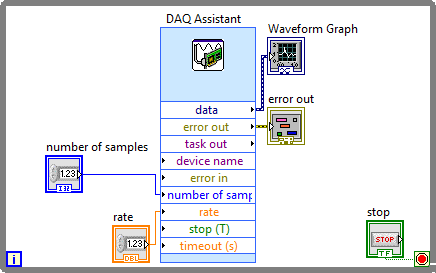
\includegraphics[width=0.8\textwidth]{pic/daq.png}
	\caption{Diese Abbildung stellt das Express-VI "DAQ-Assistant" dar. Darauf sind die verschiedenen Ein- und Ausgänge zu sehen.}
	\label{fig:daq}	
\end{figure}
Lediglich die Anzahl der Datenpunkte und die Messrate mussten dem DAQ-Assistant geliefert werden damit ein Waveform-Graph aus dem Array, welches der "data"-Ausgang ausgab, das Bild in Abb. \ref{fig:daq_sig} erzeugt werden konnte. 
\begin{figure}[ht]
	\centering
	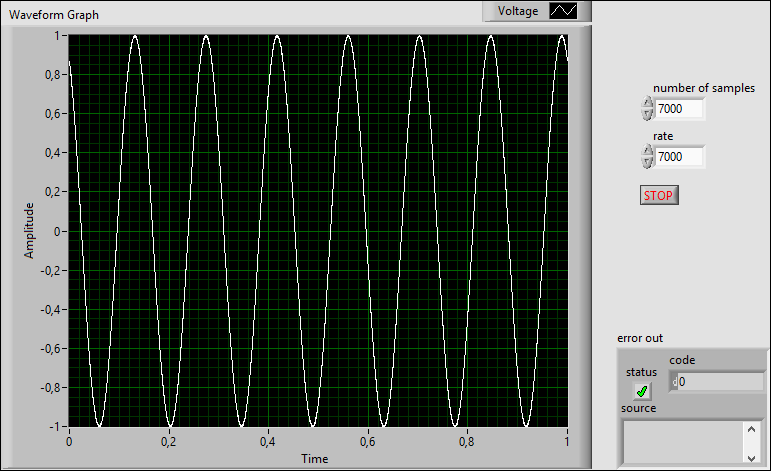
\includegraphics[width=\textwidth]{pic/daq_sig.png}
	\caption{Diese Abbildung stellt das Frontpanel eines VIs mit dem DAQ-Assistant und Controls für Messrate und Anzahl der Datenpunkte dar.}
	\label{fig:daq_sig}	
\end{figure}
Das aufgezeichnete Signal stimmte mit dem überein, was an dem Funktionsgenerator eingestellt wurde.


\newpage
\subsection{Programmieren einer eigenen Messstruktur}

Da lediglich eine Anzeige des gemessenen Signals oft nicht reicht, musste eine Messstruktur programmiert werden, die den Umfang des DAQ-Assistants übersteigt und weiter manuell angepasst werden kann.
	
\

Aufgrund von Problemen bei Wartungsarbeiten ließen sich die Computer jedoch gegen Mittag nicht mehr bedienen, weswegen das Fertigstellen des Programms auf den dritten Tag verschoben wurde. 
Zur Vorbereitung für das Weiterarbeiten wurden thematisch noch die Fouriertransformation zur Spektralanalyse, so wie das Abtasttheorem für eine richtige Messung angesprochen.
	
\


	}{}
	\IfFileExists{tex/13_Tag3.tex}{
		
Nach Abschluss der Wartungsarbeiten wurde die Arbeit an der Messstruktur fortgesetzt.
Abb. \ref{fig:messstruktur} stellt das Endprodukt für diesen Aufgabenteil dar.
\newpage
\thispagestyle{empty}
\begin{figure}[H]
	\centering
	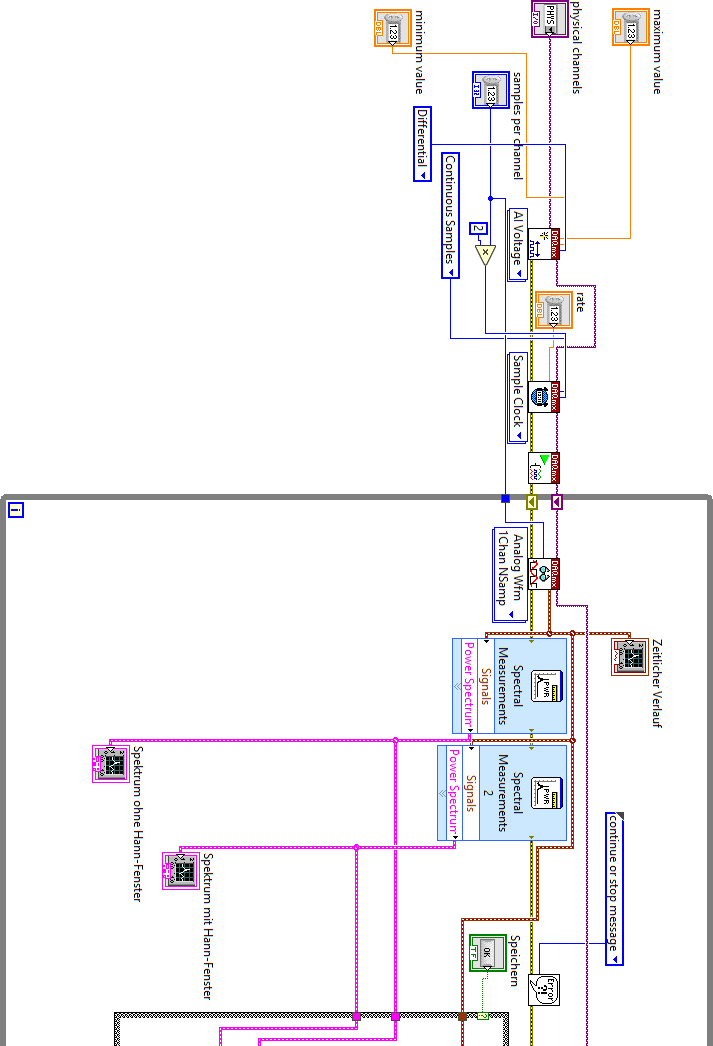
\includegraphics[width=\textwidth]{pic/messstruktur1.png}	
\end{figure}

\begin{figure}[H]
	\centering
	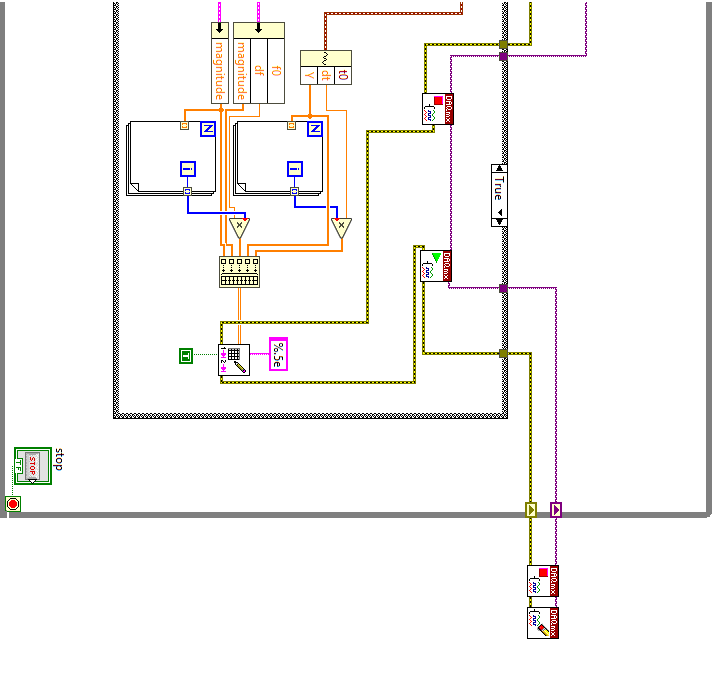
\includegraphics[width=\textwidth]{pic/messstruktur2.png}	
	\caption{LabVIEW VI zur Messung, Spektralanalyse und Speicherung eines eingehenden Signals.}
	\label{fig:messstruktur}
\end{figure}

\thispagestyle{empty}
Ähnlich zu dem DAQ-Assistant sind hier die Eingänge für Anzahl der Datenpunkte und Messrate vertreten.
Die VIs, welche die Funktionen des DAQ-Assistants ersetzen sollen sind die DAQmx-VIs, welche in Reihe geschaltet werden.
Als Eingang in das erste DAQmx-VI wir der Kanal übergeben von dem das Signal empfangen werden soll, welcher hier "physical channel" heißt.
Bei dem verwendeten Computer handelte es sich bei diesem Kanal um "Dev3/ai0".
Da Spannungen im differentiellen Modus gemessen werden sollten wurden "AI Voltage" und "Differential" als Modus bzw. konstanter Eingang an das DAQmx-VI gelegt. 
Um die gemessene Spannungen variabel zu begrenzen wurden zusätzlich Controls angebracht.
Die Benennung dieser mit "minimum value" und "maximum value" entstammt der voreingestellten Namen der Eingänge des DAQmx-VIs.
In einer späteren Version wurden die englischen Namen durch deutsche ersetzt.
Von den Ausgängen dieses VIs gehen nur der Signalkanal und ein Fehlerkanal durch, welche sich von hier aus bis ans Ende der Messstruktur durch alle DAQmx-VIs ziehen.
	
\

Das zweite DAQmx-VI dient als Taktgeber für die Aufnahme des Signals, deswegen der Modus "Sample Clock".
Ihm werden einerseits der Signalkanal und der Fehler übergeben, andererseits auch die Messrate "rate" und die doppelte Anzahl der Datenpunkte "samples per channel", damit der CPU weniger ausgelastet wird. 
Mit dem letzten und konstanten Eingang "Continuous Samples" wird festgelegt, wie die Daten aufgenommen werden.
Da der Funktionsgenerator kontinuierlich ein Signal ausgibt, soll auch so lange getaktet werden, bis der Nutzer das Programm beendet.
	
\

Das nächste DAQmx-VI ist nur für den Start des Messvorgangs zuständig.
Von dort aus geht es in eine while-Schleife mit Stopp-Knopf, damit das Programm jederzeit von dem Benutzer beendet werden kann, ohne dass ein Stopp von LabVIEW erzwungen werden muss.
In dieser while-Schleife ist das erste Element ein weiteres DAQmx-VI.
Dieses ist für das Lesen des Signals mit den vorgegebenen Parametern des Taktgebers verantwortlich.
Es gibt ein dynamisches Array der Messdaten aus, welches mit Hilfe eines Waveform-Graphen auf der Frontplatte dargestellt werden kann.  
Des Weiteren wird die Ausgabe für eine Spektralanalyse über zwei verschiedene Express-VIs genutzt. 
Dabei wird bei einem mit dem sogenannten Hann-Fenster gearbeitet und bei dem anderen ohne.
Das Hann-Fenster dient zur Manipulation der Messdaten, um die vorkommenden nicht ganzzahligen Frequenzen schärfer im Frequenzbild darzustellen, um den Leakage-Effekt zu unterdrücken, auf den später noch genauer eingegangen wird.
	
\

Neben den Daten verläuft auch das Fehlerkabel durch die Express-VIs. 
Falls ein Fehler in dem Programm auftritt dann wird aufgrund des VIs mit der Sprechblase eine Fehlermeldung ausgegeben und der Nutzer wird gefragt, ob das Programm weiterlaufen oder gestoppt werden soll.
	
\

Um die ermittelten Daten für das Zeitbild und das Frequenzbild zu speichern wird die Case-Struktur nach der Spektralanalyse eingebaut.
Wird auf den Speicherknopf auf dem Frontpanel gedrückt, so wird der in Abb. \ref{fig:messstruktur} dargestellte Fall durchgeführt.
Andernfalls der in Abb. \ref{fig:messstruktur_case} dargestellte Fall, in dem das Programm einfach weiterläuft.
\begin{figure}[H]
	\centering
	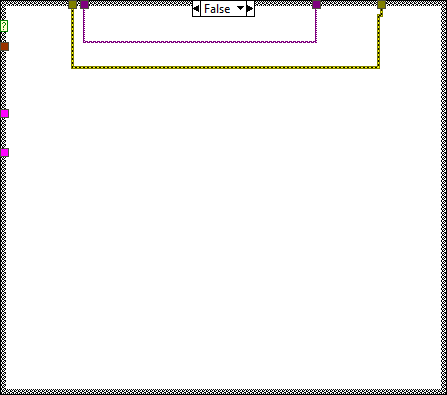
\includegraphics[width=0.5\textwidth]{pic/messstruktur_case.png}	
	\caption{Case der Messstruktur VI für den Fall, dass nicht gespeichert werden soll.}
	\label{fig:messstruktur_case}
\end{figure}

Im Falle des Speicherns hingegen wird das Lesen der Daten über ein DAQmx-VI angehalten, damit überhaupt ein fester Datensatz gespeichert werden kann.
Um die Daten zu erhalten werden das Signal des Zeitbildes und der Frequenzbilder in Waveform-Builder gegeben um die einzelnen Parameter zu erhalten.
Damit die Zeit $t_i$ und die Frequenz $f_i$ dargestellt werden können, werden die Differentiale d$t$ und d$s$ über for-Schleifen $i$ mal aufaddiert.
Aus diesen Zeiten und Frequenzen werden mit ihren jeweiligen Amplituden (\si{\volt} im Zeitbild und \si{\decibel} im Frequenzbild, mit und ohne Hann-fenster) in ein Array gegeben und in ein VI gegeben, welches eine Datei ausgibt, in dem das Array mit $i$ Zeilen und den fünf Spalten für die einzelnen Parametern ausgegeben wird.
An diesem VI lässt sich auch das Format der Daten darstellen, hier wurde "\%.5e" gewählt für eine Ausgabe wie in Tab. \ref{tab:speichern} für die exponentielle Schreibweise und fünf Nachkommastellen.	
\begin{table}[ht]
	\centering
	\begin{tabular}{S S S S S}
		
		\text{0,00000E+0} &	\text{0,00000E+0} &	\text{1,21707E+0} &	\text{-4,15539E+1} &	\text{-5,78080E+1}\\
		\text{1,00000E-3} &	\text{1,00000E+0} &	\text{-6,34577E-1} &	\text{-3,99954E+1} &	\text{-6,09291E+1} \\
		\text{2,00000E-3} &	\text{2,00000E+0} &	\text{-2,24044E+0} &	\text{-4,00174E+1} &	\text{-9,43314E+1} \\
		\text{3,00000E-3} &	\text{3,00000E+0} &	\text{-2,98161E+0} &	\text{-4,00395E+1} &	\text{-8,78620E+1} \\
		$\colon$ \\		
		$\colon$ \\		
	\end{tabular}
	\caption{Beispielausgabe nach Nutzung der Speicherfunktion der Messstruktur.}
	\label{tab:speichern}
\end{table}
Eine automatische Benennung der Spalten ist hierbei nicht möglich, weswegen verfolgt werden muss welcher Wert an welcher Stelle in das Array eingefügt wird.
	
\

Danach wird die Schleife wiederholt bis sie durch Betätigen des Stopp-Knopfes verlassen wird.
Nach zwei weiteren DAQmx-VIs wird das Programm dann beendet.



\subsection{Abtastung mit der Messstruktur}

Mit der vorerst fertigen Messstruktur sollte nun abgetastet werden.
Die Abbildungen \ref{fig:abtast_1kHz} bis \ref{fig:abtast_250,5Hz} stellen verschiedene Fälle dar.
Der Verlauf in Abb. \ref{fig:abtast_1kHz} stellt den Fall der Unterabtastung dar.
Hierbei entspricht die Frequenz der Messung mit der Signalfrequenz des Funktionsgenerator überein.
Um das Abtasttheorem zu erfüllen, müsste jedoch mit mindestens der doppelten Frequenz abgetastet werden, weswegen hierbei keine Schwingung sondern nur ein annähernd linearer Verlauf im Zeitbild zu erkennen ist.
Im Falle einer Messung mit exakt gleicher Frequenz wäre jedoch ein konstanter Verlauf zu erwarten, dies schließt auf einen Unterschied zwischen der Frequenz des Funktionsgenerators und der Messrate, obwohl beide auf den selben Wert eingestellt waren.
	
\

Abb. \ref{fig:abtast_5Hz} verdeutlicht die Ungenauigkeit bei der Messung weiter.
Hier war der Funktionsgenerator auf \SI{5}{\hertz} eingestellt, gemessen wurde jedoch ein breites Spektrum an Frequenzen, bei denen die am stärksten vorkommenden Frequenzen zwischen \SIrange{5}{6}{\hertz} liegen.
	
\

Insbesondere die Darstellung im Frequenzbild von Signalen mit nicht ganzzahligen Frequenzen stellt bei vorliegender Messtechnik ein Problem dar.
Vergleicht man die Abbildungen \ref{fig:abtast_250Hz} und \ref{fig:abtast_250,5Hz}, so ist bereits im Zeitbild zu erkennen, dass im nicht ganzzahligen Fall, bei einer Frequenz, die lediglich \SI{0,5}{\hertz} über der anderen liegt ein deutlich anderes Bild zu sehen ist, obwohl es sich bei beiden um einfache Sinusschwingungen mit jeweils nur eine Frequenz handeln sollte.
Aufgrund der groß gewählten Frequenzen ist die Sinusform in Abb. \ref{fig:abtast_250Hz} kaum zu erkennen, jedoch lässt sich anhand der Amplituden ein Muster erkennen, welches einem einfachen Sinus deutlich mehr ähnelt als das in Abb. \ref{fig:abtast_250,5Hz}.
	
\

Betrachtet man nun die Frequenzbilder, so fällt zunächst im Fall ohne Hann-Fenster auf, dass bei dem \SI{250}{\hertz}-Signal eine Frequenz noch recht deutlich heraus sticht.
Bei dem \SI{250,5}{\hertz}-Signal weitet sich dieser Frequenzpeak jedoch auf und die Frequenz des Signals lässt sich somit deutlich schlechter erfassen.
Dies nennt man Leakage-Effekt.
Um dieses "Ausschmieren" zu verhindern, kann das Signal mit Hilfe einer sogenannten Fensterfunktion manipuliert werden.
In den Abbildungen werden hier Hann-Fenster verwendet.
Vergleicht man die Frequenzbilder mit Hann-Fenster in den Abbildungen \ref{fig:abtast_250Hz} und \ref{fig:abtast_250,5Hz} so fällt auf, dass der Leakage-Effekt deutlich geschwächt auftritt, dafür aber verstärktes Rauschen in den umliegenden Frequenzbereichen zu erkennen ist.
Dieses Rauschen jedoch liegt weit unter dem gewünschten Frequenzpeak bei ca. \SI{-80}{\decibel} und ist demnach zu vernachlässigen.

\begin{figure}[H]
	\centering
	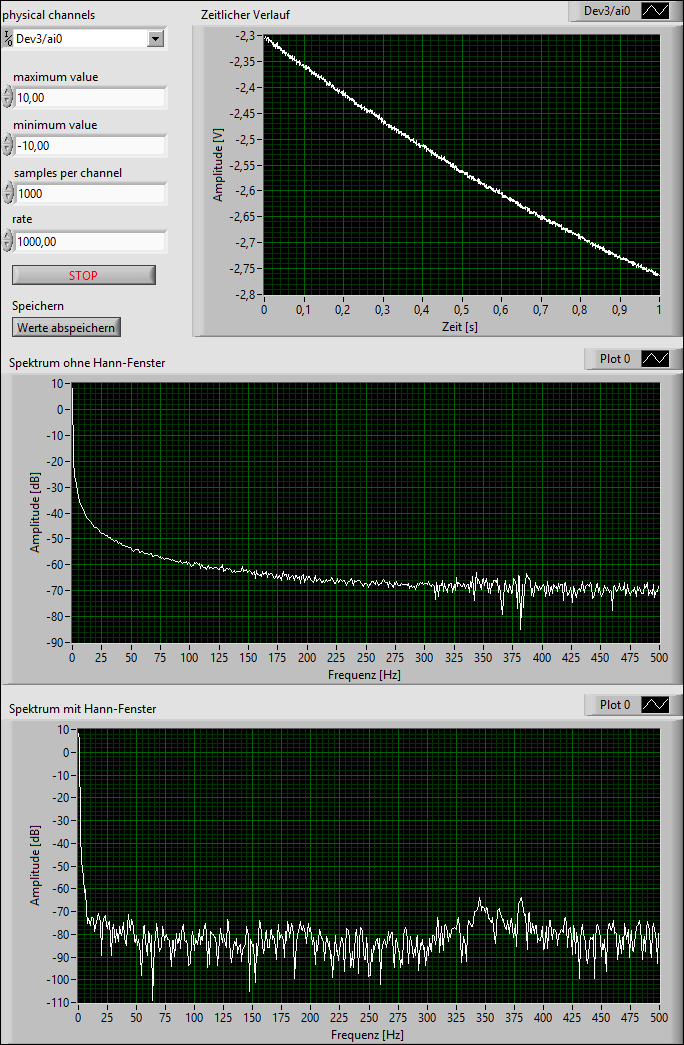
\includegraphics[width=0.85\textwidth]{pic/abtast_1kHz.png}	
	\caption{Frontpanel der Messstruktur bei eingehendem Sinussignal mit Frequenz \SI{1}{\kilo\hertz} und voreingestellten Parametern für Messrate etc.}
	\label{fig:abtast_1kHz}
\end{figure}

\begin{figure}[H]
	\centering
	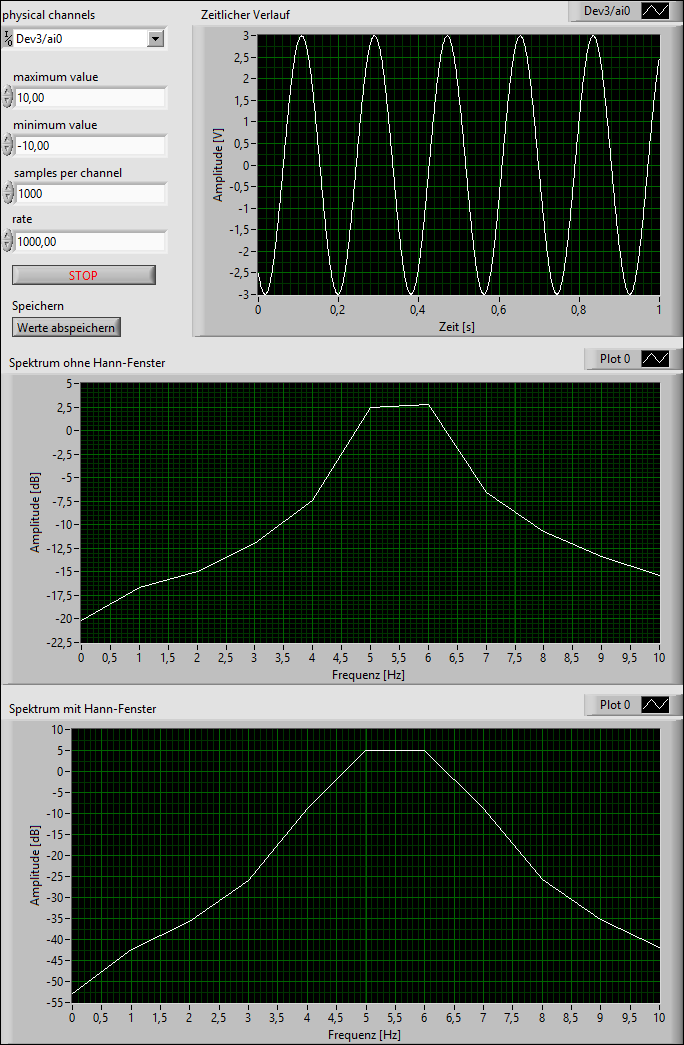
\includegraphics[width=0.85\textwidth]{pic/abtast_5Hz.png}	
	\caption{Frontpanel der Messstruktur bei eingehendem Sinussignal mit Frequenz \SI{5}{\hertz} und voreingestellten Parametern für Messrate etc.}
	\label{fig:abtast_5Hz}
\end{figure}
	
\begin{figure}[H]
	\centering
	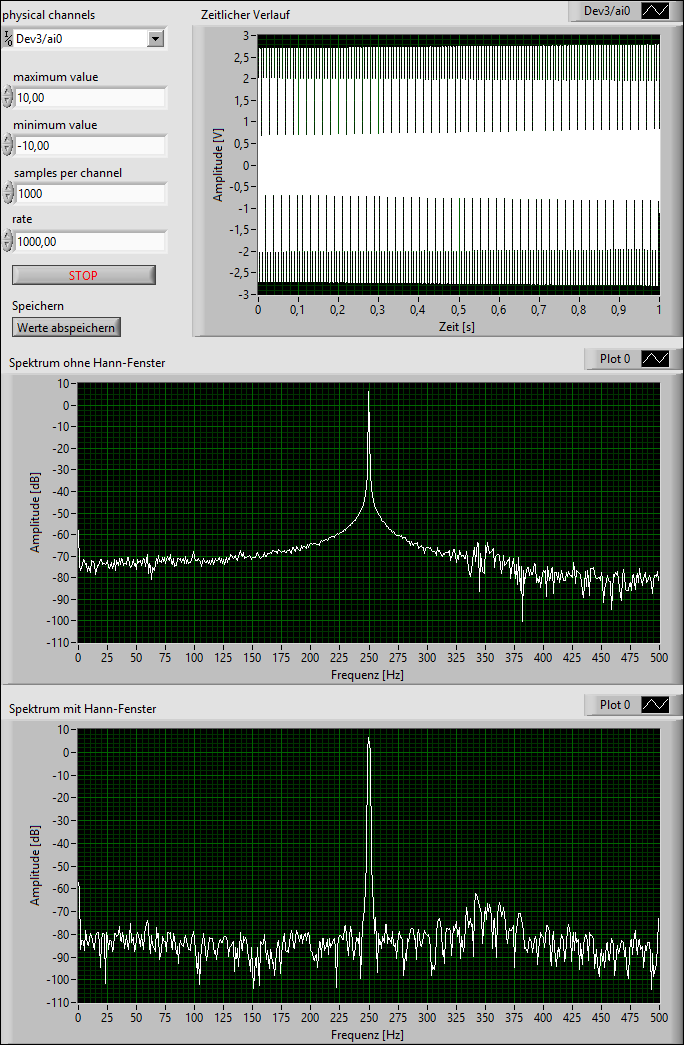
\includegraphics[width=0.85\textwidth]{pic/abtast_250Hz.png}	
	\caption{Frontpanel der Messstruktur bei eingehendem Sinussignal mit Frequenz \SI{250}{\hertz} und voreingestellten Parametern für Messrate etc.}
	\label{fig:abtast_250Hz}
\end{figure}

\begin{figure}[H]
	\centering
	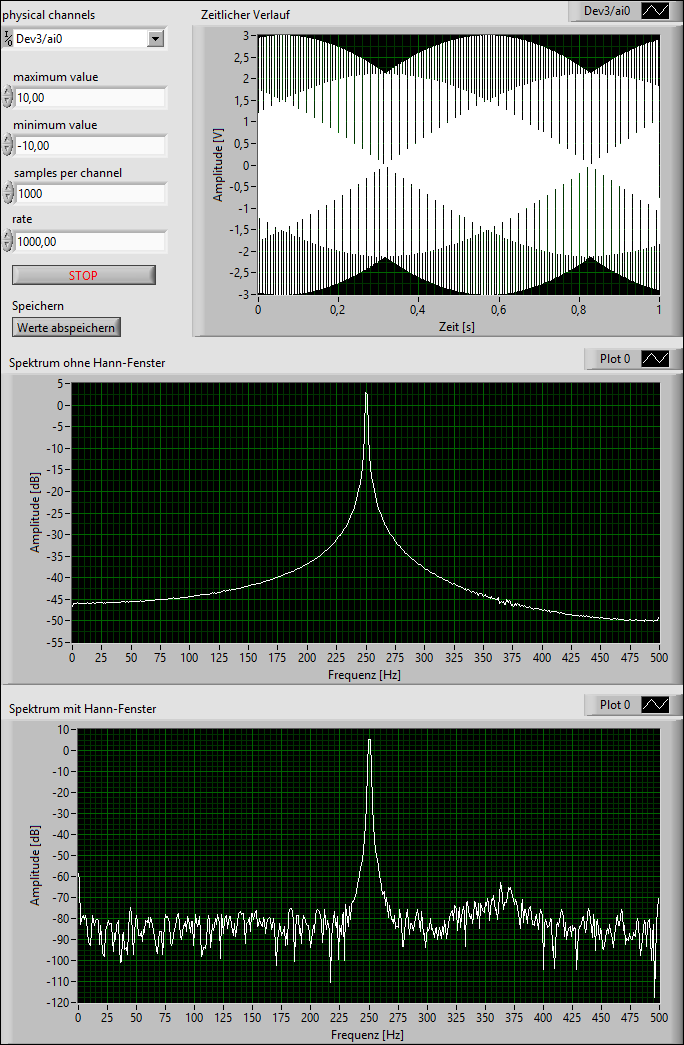
\includegraphics[width=0.85\textwidth]{pic/abtast_250,5Hz.png}	
	\caption{Frontpanel der Messstruktur bei eingehendem Sinussignal mit Frequenz \SI{250,5}{\hertz} und voreingestellten Parametern für Messrate etc.}
	\label{fig:abtast_250,5Hz}
\end{figure}

\newpage
\section{Modulation}

Als nächstes sollte der Funktionsgenerator durch die computereigene Soundkarte ersetzt werden.
Um einen Schritt weiter zu gehen, sollte das Signal, welches der Soundkarte über ein LabVIEW VI übergeben wird, amplitudenmoduliert sein.



\subsection{Amplitudenmodulation}

Das VI, welches ein amplitudenmoduliertes Signal erzeugt und von der Soundkarte ausgeben lässt ist in Abb. \ref{fig:am} dargestellt.
Die VIs, welche für die Soundkartenausgabe zuständig sind, sind mit einem Lautsprechersymbol gekennzeichnet. 
Wie auch bei der Messtruktur verläuft von dem ersten dieser VIs eine Fehlerleitung, damit eine Fehlermeldung ausgegeben werden kann, falls in dem Programm ein Fehler auftritt.
Da auch hier ein kontinuierliches Signal gesendet werden soll, wird der Modus "Continuous Samples" für die Ausgabe festgelegt.
Bei den drei Konstanten welche neben dem Modus in das Sound-VI gegeben werden handelt es sich um Frequenz, Anzahl der Kanäle und Bits.
Mit den gewählten Werten von \SI{44100}{\hertz}, einem Kanal und 16 Bits wird der Ton im Mono-Format und mit CD-Qualität ausgegeben, welche die eingebaute Soundkarte unterstützt.
Das Sound-VI nach der Übergabe der Parameter startet die Ausgabe und von dort wird die Schleife betreten, in der das Signal entsteht.
Zu erkennen sind bereits Controls für das zu modulierende Signal, wie auch für den Träger.
Hierzu liegt dem Aufbau folgende Formel zu Grunde:
\begin{align}
	\label{eq:AM1} S_\text{AM}(t) &= (m \cdot S(t) + 1) \cdot T(t) \\
	\label{eq:AM2} \text{mit dem Signal} \quad S(t) &= A_1 \cdot \sin{(2\pi f_1 t)} + A_2 \cdot \sin{(2\pi f_2 t)}\\
	\label{eq:AM3} \text{und dem Träger} \quad T(t) &= s_\text{T} \cdot \sin{(2\pi f_\text{T} t)}.
\end{align} 

\

Aufgrund der Beschränkung der Soundkarte auf Signale mit maximaler Amplitude von einem Volt, wird der Modulationsgrad $m$ variabel gehalten, aber $s_\text{T}$ auf $\frac{1}{mA_1 + mA_2 + 1}$ normiert. 
$A_{1/2}$ sind dabei die Amplituden der beiden Sinusschwingungen aus denen das zu modulierende Signal besteht und $f_{1/2}$ die jeweiligen Frequenzen, analog $f_\text{T}$ die Frequenz für den Träger.

\newpage
\thispagestyle{empty}
\begin{figure}[H]
	\centering
	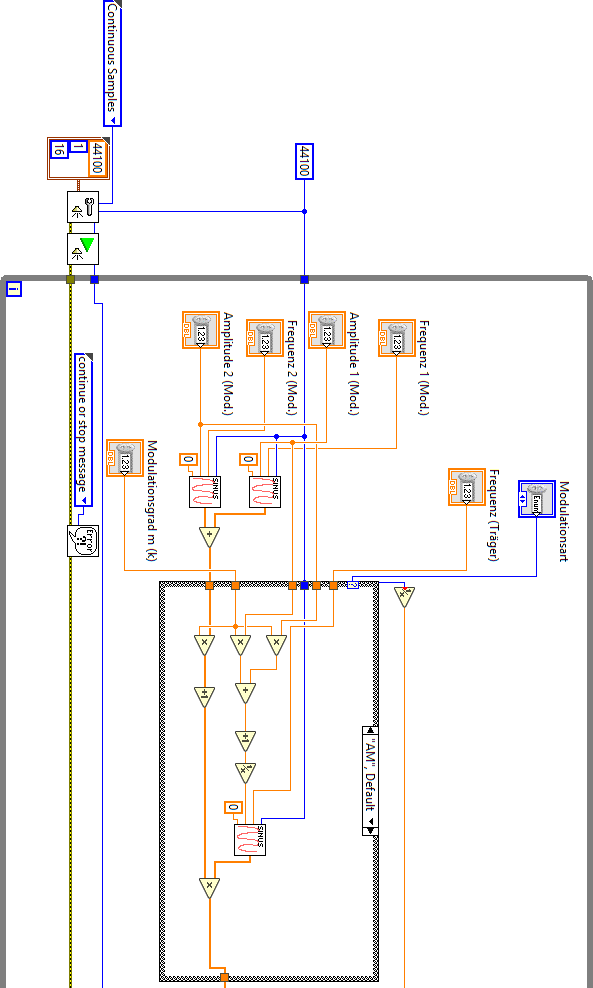
\includegraphics[width=0.95\textwidth]{pic/am1.png}
\end{figure} 

\begin{figure}[H]
	\centering
	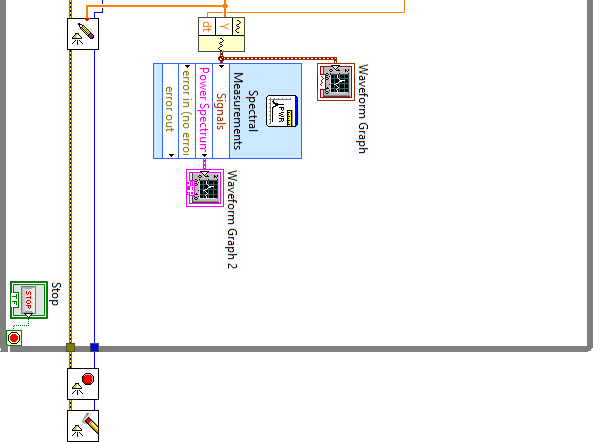
\includegraphics[width=0.95\textwidth]{pic/am2.png}
	\caption{LabVIEW VI zur Erstellung eines amplitudenmodulierten Signals, welches von der Soundkarte ausgegeben und auf dem Frontpanel einstellbar und graphisch dargestellt wird.}
	\label{fig:am}	
\end{figure} 

\thispagestyle{empty}
Das Signal $S(t)$ wird wie in Abb. \ref{fig:am} zu erkennen durch zwei der zuvor geschriebenen Sinus VIs verwirklicht.
Zur besseren Aufnahme werden an dieser Stelle genau so viele Datenpunkte gewählt wie auch für die Sound VIs. 
Analog zu der Frequenz hier 44100 Datenpunkte.
Wie in der obigen Formel zu erkennen, werden die Phasen der Signale vernachlässigt und einfach gleich null gesetzt.
Die eigentliche Modulation, also der Übergang von $S(t)$ zu $S_\text{AM}(t)$ findet in der Case-Struktur statt.
Bei der Abbildung handelt es sich um das Endprodukt mit zudem eingebauter Frequenz- und Phasenmodulation zwischen denen hier unterschieden werden kann.
Auf die anderen Cases wird später eingegangen, da diese erst im Nachhinein in das Modulations-VI hinzugefügt wurden.
	
\

\

Zurück zu dem AM-Case: Hier sind die Rechnungen aus den Gleichungen \ref{eq:AM1} und \ref{eq:AM3} mit normierter Amplitude nachgestellt.
Das Sinus-VI in dem Case stellt hierbei das Trägersignal dar, welches ebenfalls die Zahl der Datenpunkte von 44100 und Phase null besitzt.
Zur Darstellung des modulierten Signals sind zudem ein Waveform-Builder und zwei damit verbundene Graphen hinzugefügt worden, damit man dieses im Zeit- und Frequenzbild auf dem Frontpanel betrachten kann.
Natürlich verläuft das Signal nicht nur in den Waveform-Builder sondern auch in das Sound-VI, welches für die Ausgabe des eingehenden Signals über die Soundkarte führt.
An dieser Stelle jedoch wurde der Ausgang zunächst falsch verkabelt, weswegen nicht das modulierte Signal ausgegeben wurde.
Dieses Problem wurde erst am vierten und letzten Tag bei Erweiterung von Frequenz- und Phasenmodulation behoben.
	
\

Wie auch bei der Messstruktur wird der Vorgang solange wiederholt bis der Stopp-Knopf auf dem Frontpanel gedrückt wird.  
In Abbildung \ref{fig:am_example} ist dieses Frontpanel für ein Beispielsignal dargestellt.

\begin{figure}[H]
	\centering
	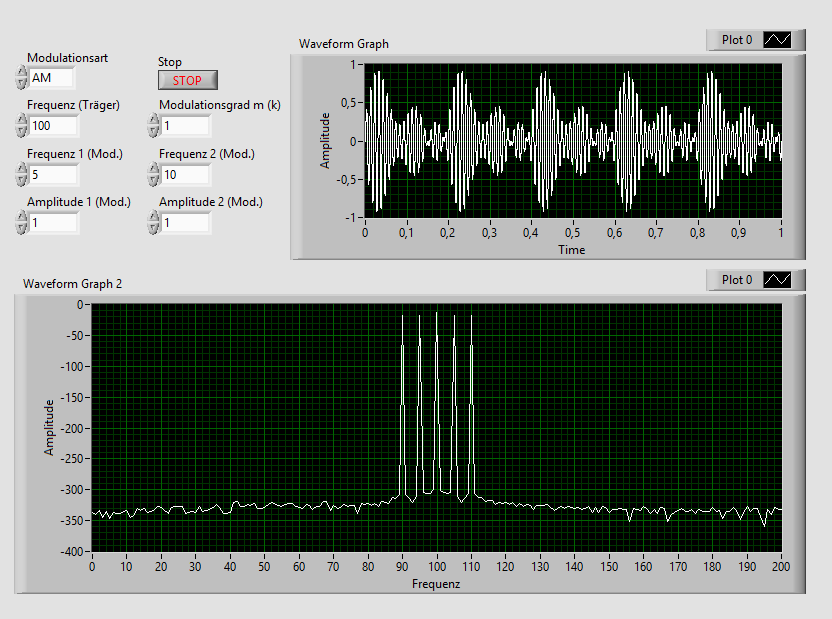
\includegraphics[width=0.8\textwidth]{pic/am_example.png}
	\caption{Frontpanel des Modulation-VIs bei AM mit Beispielsignal und einstellbaren Parametern.}
	\label{fig:am_example}	
\end{figure} 

Zu erkennen sind hier im Frequenzbild die Trägerfrequenz und die von der Amplitudenmodulation üblichen Seitenbänder links und rechts von der Trägerfrequenz pro Frequenz die im zu modulierenden Signal auftritt, sowie auch der schwebungsähnliche Verlauf im Zeitbild.
Im Anhang (Abschnitt \ref*{sec:anhang}) sind weitere Beispiele verzeichnet.



\subsection{Erweiterung der Messstruktur}

Damit das nun modulierte Signal auch wieder demoduliert werden kann, musste die Messstruktur erweitert werden.
Für die Amplitudenmodulation wurden hier drei verschiedene Arten der Demodulation integriert, von denen eine ausgewählt werden kann.
Die Erweiterung von Abb. \ref{fig:messstruktur} ist in Abb. \ref{fig:messstruktur_dam} dargestellt.
	
\

Bei den verschiedenen Demodulationsverfahren handelt es sich um die Quadratur, die Betragsbildung und die Multiplikation mit dem Träger, welche jedoch erst im Nachhinein am Morgen des vierten Tages hinzugefügt wurde.
Um auch hier zu unterscheiden wurde eine Case-Struktur angelegt, bei der auch "keine Demodulation" eine Option ist.
Der Fall der Quadratur ist bereits in Abb. \ref{fig:messstruktur_dam} dargestellt.
Das Signal wird dabei einfach quadriert.
Analog dazu wird bei der Betragsbildung einfach ein VI für den Betrag eingeschoben und bei keiner Demodulation die Kabel ohne weiteres durch den Case gezogen (vgl. Abb. \ref{fig:messstruktur_dam_case}). 
Da nach den Rechenoperationen auch noch Frequenzen im Bereich doppelter Trägerfrequenz auftauchen, müssen diese gefiltert werden.
Dies lässt sich leicht mit einem Tiefpass verwirklichen, solange das Verhältnis zwischen Trägerfrequenz und der des Ursprungssignals $f_\text{T} >> f_{1/2}$ gilt.
	
\

Vor und nach dem Tiefpass wurden weitere Graphen für Zeit- und Frequenzbild eingefügt, um die einzelnen Schritte der Signalverarbeitung auch visuell auf dem Frontpanel darzustellen.
Ansonsten ist das VI im wesentlichen das gleiche wie in Abb. \ref{fig:messstruktur}, nur die Speicherfunktion wurde noch um die zwei weiteren Datensätze nach Demodulation und nach Tiefpass erweitert.

\newpage
\pagestyle{empty}

\begin{figure}[H]
	\centering
	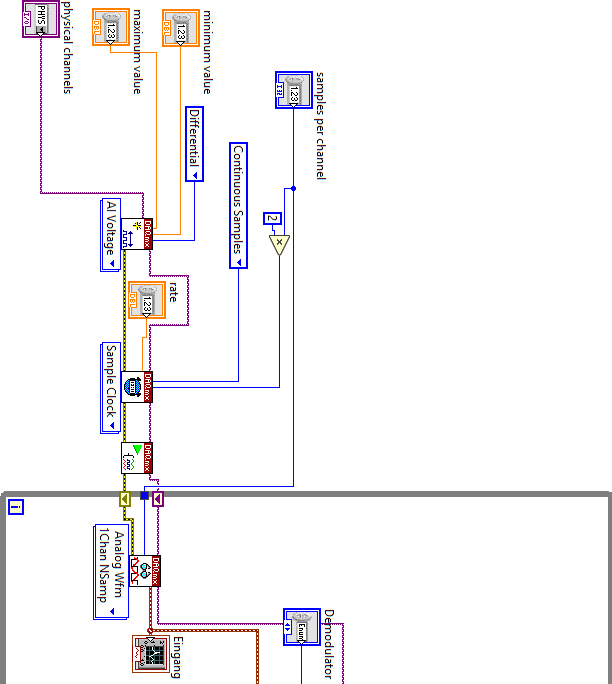
\includegraphics[width=\textwidth]{pic/messstruktur_dam1.png}
\end{figure} 

	\begin{figure}[H]
	\centering
	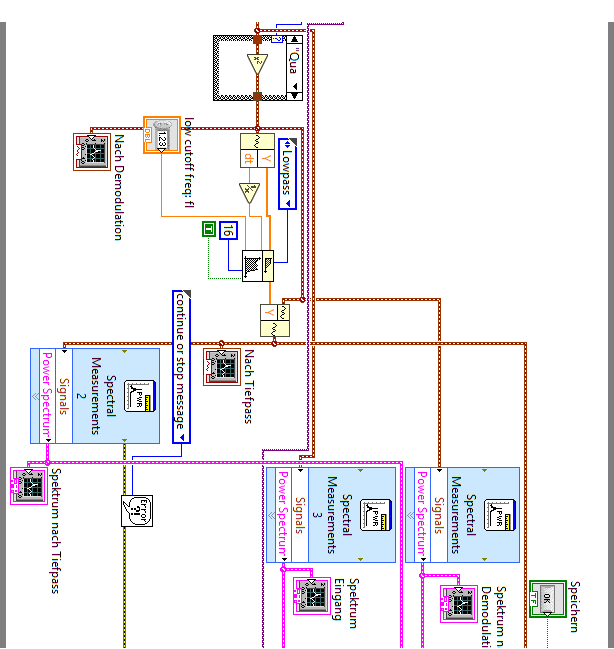
\includegraphics[width=\textwidth]{pic/messstruktur_dam2.png}
\end{figure} 

\begin{figure}[H]
	\centering
	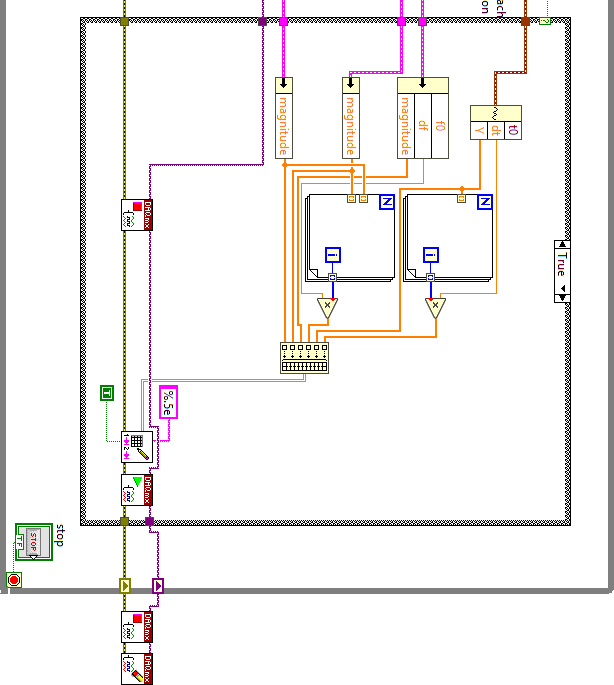
\includegraphics[width=\textwidth]{pic/messstruktur_dam3.png}
	\caption{Frontpanel des Modulation-VIs bei AM mit Beispielsignal und einstellbaren Parametern.}
	\label{fig:messstruktur_dam}	
\end{figure} 

\pagestyle{headings}

\begin{figure}[H]
	\centering
	\begin{subfigure}[c]{0.45\textwidth}
		\centering
		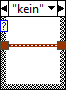
\includegraphics[width=0.3\textwidth]{pic/messstruktur_dam_case1.png}
		\subcaption{Case für den Fall ohne Demodulation.}
	\end{subfigure}
	\begin{subfigure}[c]{0.45\textwidth}
		\centering
		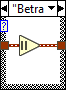
\includegraphics[width=0.3\textwidth]{pic/messstruktur_dam_case2.png}
		\subcaption{Case für den Fall von Demodulation über Betragsbildung.}
	\end{subfigure}	
	\caption{Alternative Fälle für den Case für die Demodulationsart in Abb. \ref{fig:messstruktur_dam}.}
	\label{fig:messstruktur_dam_case}	
\end{figure}

\

Wie bereits zuvor erwähnt, war das Ende der Modulations-VI zunächst falsch verkabelt.
Die Darstellungen für das Frontpanel der erweiterten Messstruktur wurden deshalb mit Hilfe eines von dem Funktionsgenerator ausgehenden Signals aufgenommen.
Diese sind in den Abbildungen \ref{fig:dam_keine} bis \ref{fig:dam_betrag} jeweils einmal pro Demodulationsart aufgefasst.
Für alle drei Abbildungen wurde das gleiche Signal von dem Funktionsgenerator verwendet mit Modulationsfrequenz $f_1= \SI{1}{\kilo\hertz}, f_2 = \SI{0}{\hertz}$, Trägerfrequenz $f_\text{T}\SI{1}{\kilo\hertz}$ und Modulationsgrad $m = 0,03$.
Bei Abb. \ref{fig:dam_keine} entsprichen die Graphen nach der Demodulation selbstverständlich denen des Eingangssignals, da dieses nicht weiter verarbeitet wurde.
Der Tiefpass erreicht an dieser Stelle nichts.
Bei den Abbildungen \ref{fig:dam_quadrat} und \ref{fig:dam_betrag} hingegen kann man den Frequenzbildern nach der jeweiligen Demodulation entnehmen, dass nur die Frequenz des zu modulierenden Signals $f_1$, die Trägerfrequenz $f_\text{T}$ und das doppelte der Trägerfrequenz mit Seitenbändern vorliegt.
An dieser Stelle erfüllt der Tiefpass seinen Zweck und in den Frequenzbildern ist die einzige Frequenz, die nicht in dem Rauschen bei $\leq \SI{-50}{\decibel}$ untergeht gerade die gesuchte Frequenzen des zu modulierenden Signals $f_1$.

Weitere Beispiele sind auch für diese im Anhang (Abschnitt \ref{sec:anhang}) vorzufinden.

\newpage
\pagestyle{empty}
\begin{figure}[H]
	\centering
	\begin{subfigure}[c]{\textwidth}
		\centering
		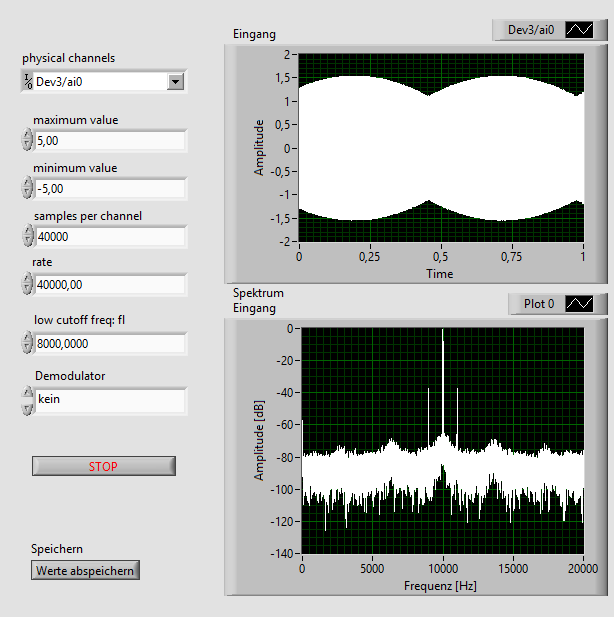
\includegraphics[width=0.7\textwidth]{pic/dam_keine1.png}
		\subcaption{Linke Seite des Frontpanels mit Parametern und Graphen für das Eingangssignal.}
	\end{subfigure}
	\begin{subfigure}[c]{\textwidth}
		\centering
		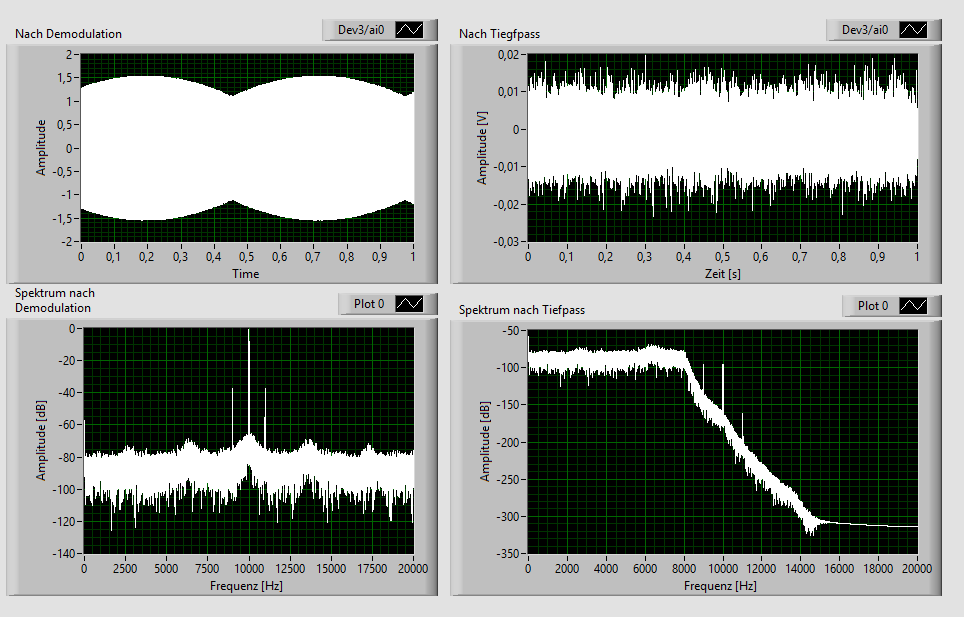
\includegraphics[width=0.9\textwidth]{pic/dam_keine2.png}
		\subcaption{Rechte Seite des Frontpanels mit Graphen für das demodulierte Signal vor und nach Tiefpass.}
	\end{subfigure}	
	\caption{Frontpanel der erweiterten Messstruktur bei eingehendem AM-Signal vom Funktionsgenerator mit Modulationsfrequenz $f_1= \SI{1}{\kilo\hertz}, f_2 = \SI{0}{\hertz}$, Trägerfrequenz $f_\text{T}\SI{1}{\kilo\hertz}$ und Modulationsgrad $m = 0,03$ ohne Demodulation.}
	\label{fig:dam_keine}	
\end{figure} 

\begin{figure}[H]
	\centering
	\begin{subfigure}[c]{\textwidth}
		\centering
		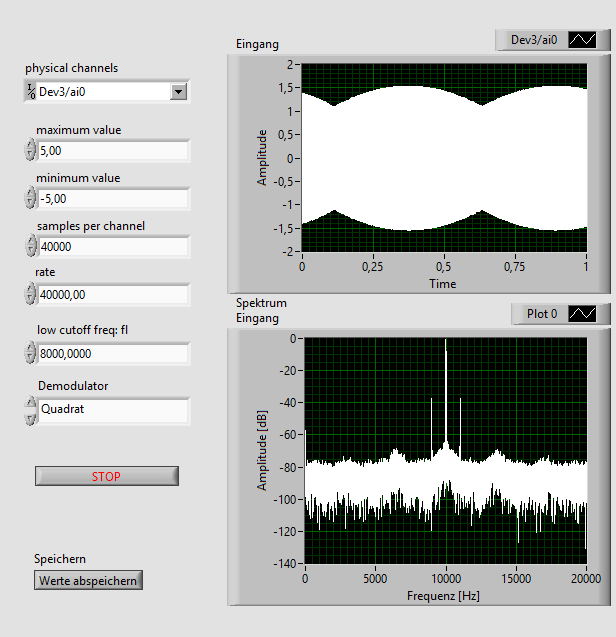
\includegraphics[width=0.7\textwidth]{pic/dam_quadrat1.png}
		\subcaption{Linke Seite des Frontpanels mit Parametern und Graphen für das Eingangssignal.}
	\end{subfigure}
	\begin{subfigure}[c]{\textwidth}
		\centering
		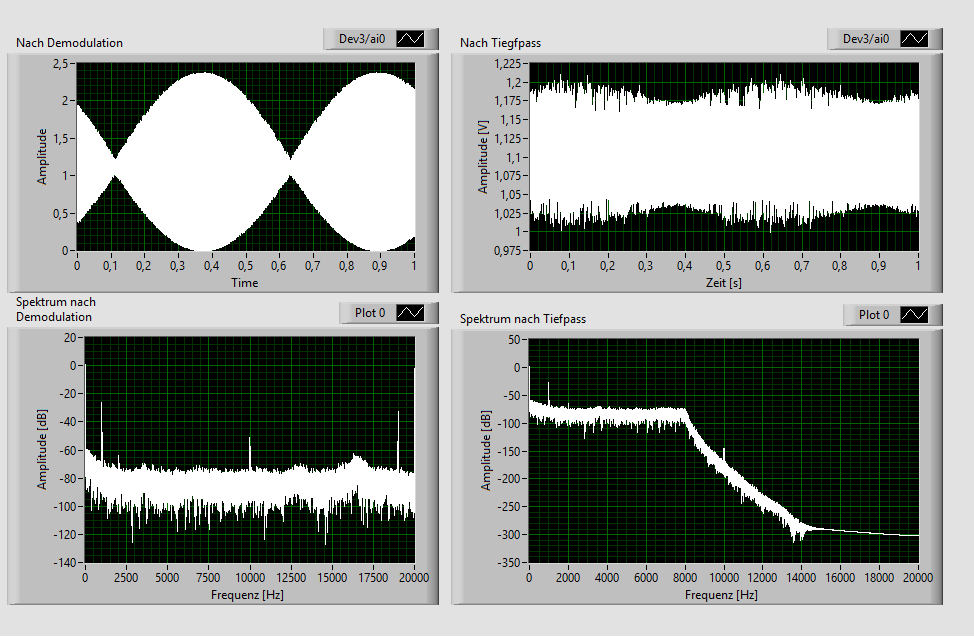
\includegraphics[width=0.9\textwidth]{pic/dam_quadrat2.png}
		\subcaption{Rechte Seite des Frontpanels mit Graphen für das demodulierte Signal vor und nach Tiefpass.}
	\end{subfigure}	
	\caption{Frontpanel der erweiterten Messstruktur bei eingehendem AM-Signal vom Funktionsgenerator mit Modulationsfrequenz $f_1= \SI{1}{\kilo\hertz}, f_2 = \SI{0}{\hertz}$, Trägerfrequenz $f_\text{T}\SI{1}{\kilo\hertz}$ und Modulationsgrad $m = 0,03$ ohne Demodulation.}
	\label{fig:dam_quadrat}	
\end{figure} 

\begin{figure}[H]
	\centering
	\begin{subfigure}[c]{\textwidth}
		\centering
		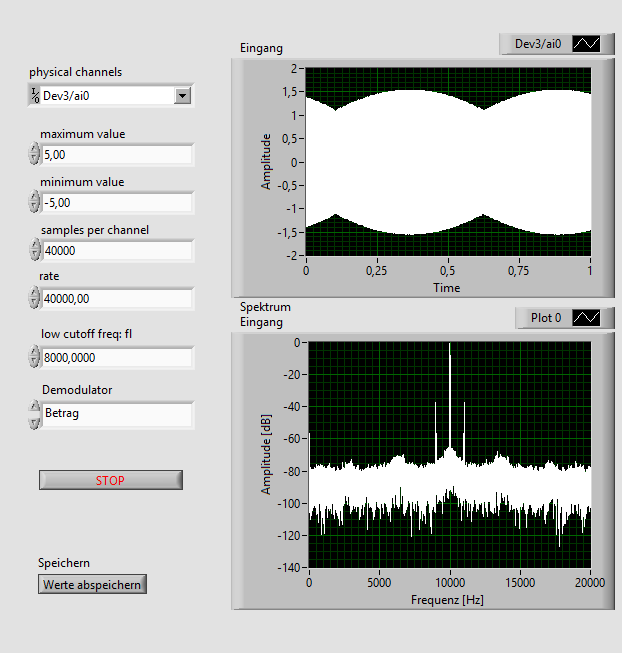
\includegraphics[width=0.7\textwidth]{pic/dam_betrag1.png}
		\subcaption{Linke Seite des Frontpanels mit Parametern und Graphen für das Eingangssignal.}
	\end{subfigure}
	\begin{subfigure}[c]{\textwidth}
		\centering
		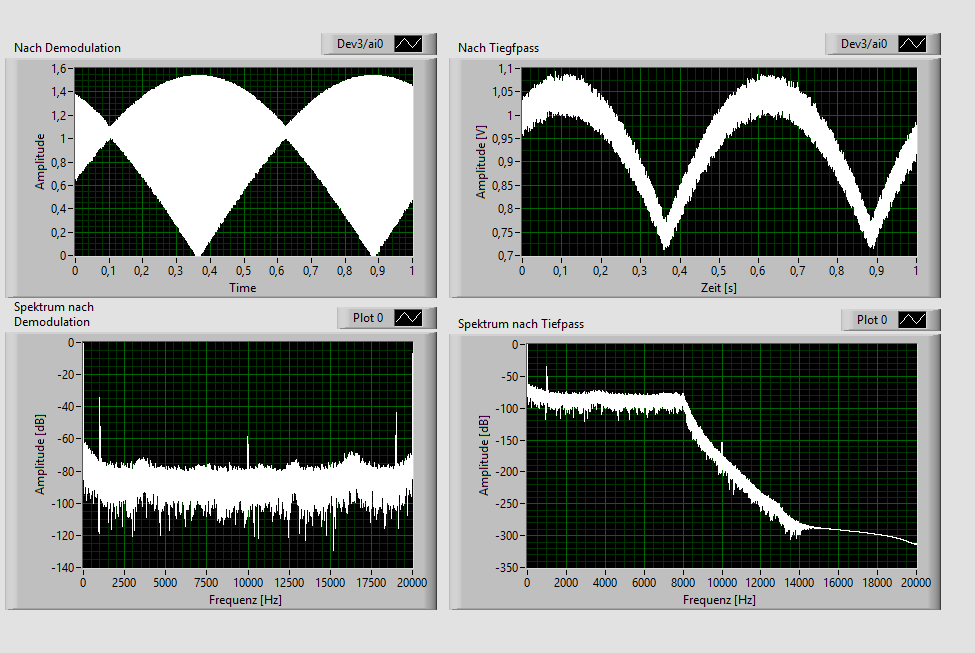
\includegraphics[width=0.9\textwidth]{pic/dam_betrag2.png}
		\subcaption{Rechte Seite des Frontpanels mit Graphen für das demodulierte Signal vor und nach Tiefpass.}
	\end{subfigure}	
	\caption{Frontpanel der erweiterten Messstruktur bei eingehendem AM-Signal vom Funktionsgenerator mit Modulationsfrequenz $f_1= \SI{1}{\kilo\hertz}, f_2 = \SI{0}{\hertz}$, Trägerfrequenz $f_\text{T}\SI{1}{\kilo\hertz}$ und Modulationsgrad $m = 0,03$ ohne Demodulation.}
	\label{fig:dam_betrag}	
\end{figure} 
	}{}
	\IfFileExists{tex/14_Tag4.tex}{
		\clearpage
		
\pagestyle{headings}
Zu Beginn des vierten Tages sollte die Messstruktur nun um die dritte Art der Demodulation, der Multiplikation mit dem Träger, erweitert werden.
Dieser neue Case ist in Abb. \ref{fig:messstruktur_dam_case3} dargestellt.
\begin{figure}[H]
	\centering
	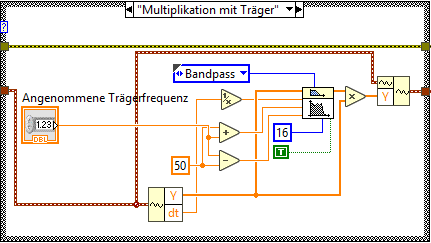
\includegraphics[width=\textwidth]{pic/messstruktur_dam_case3.png}
	\caption{Case für den Fall der  Multiplikation mit dem Träger als Demodulationsart.}
	\label{fig:messstruktur_dam_case3}	
\end{figure} 
In diesem Falle muss eine geschätzte Trägerfrequenz angegeben werden, da diese nicht einfach dem eingehenden Signal zu extrahieren ist.
Zudem muss, um das Auftreten ungewollter Seitenbänder zu unterdrücken, das Trägersignal vorher mit einem Bandpass so verändert werden, dass die Trägerfrequenz möglichst die einzige verbliebene Frequenz in dem Signal ist, sodass dann bei der Multiplikation mit dem moduliertem Signal die Trägerfrequenz wegfällt und nur die Frequenzen des Ursprungssignals $S(t)$ überbleibt.
Vollständig verschwindet die Trägerfrequenz so jedoch nicht, da auch Frequenzanteile mit doppelter Trägerfrequenz auftreten.
Diese lassen sich aber wie zuvor durch den Tiefpass hinter dem Case filtern.
Um sich gleichzeitig auch noch um den Gleichanteil, zu kümmern wird dieser Tiefpass hinter dem Case durch einen Bandpass ersetzt, was in Abb. \ref{fig:messstruktur_dafpm} in der vollständigen Messstruktur zu sehen ist.
	
\

Bevor es jedoch zu Vervollständigung der Messstruktur durch Erweiterung der Demodulation von frequenz- und phasenmodulierten Signalen kommt, war die nächste Aufgabe zunächst einmal das Modulations-VI um die beiden fehlenden Arten der Modulation zu erweitern.
An dieser Stelle ließ sich dann auch der Fehler in der Verkabelung feststellen und die Soundkarte konnte nun die Position des Funktionsgenerators ersetzen.
Dabei wurde der Audio-Ausgang des Rechners mit dem ADC dort verbunden, wo vorher der Funktionsgenerator angeschlossen war.
	
\

Die Erweiterung des Modulations-VI um Frequenz- und Phasenmodulation belief sich auf die in Abb. \ref{fig:am} nicht dargestellten Cases.
Diese sind in der Abbildung \ref{fig:fmpm} dargestellt.
Für diese wurden folgende Formeln herangezogen und in LabVIEW modelliert:
\begin{align}
	\label{eq:FM} S_\text{FM}(t) &= \cos{(2\pi[f_\text{T}t + k \cdot \int_{-\infty}^{t}{S(\tau)\dd{\tau}}])} \\
	\label{eq:PM} S_\text{PM}(t) &= \cos{(2\pi[f_\text{T}t + k \cdot S(t)])}.
\end{align} 
Wie auch bei dem Abspeichern wird eine for-Schleife verwendet um die Zeit $t_i$ über den Kehrwert der Messfrequenz in $i$ Schritten zu konstruieren.
Der Modulationsgrad $m$ aus der Amplitudenmodulation entspricht hier dem $k$ aus der Formel.
Im Wesentlichen unterscheiden sich der Fall der Frequenzmodulation von der Phasenmodulation nur dadurch, dass das zu modulierende Signal vor weiteren Rechenoperationen noch integriert wird.
Da die Amplitude für das ausgehende Signal für den Modulationsprozess hier keine große Rolle spielt, solange sie ungleich null ist, wird diese hier auf eins gesetzt.
Durch einfache Rechenoperationen wird das Argument des Kosinus aufgestellt und dann in die Funktion gegeben.
		
\
	
Jeweils ein Beispiel des Frontpanels für die beiden neuen Modulationsverfahren ist in Abb. \ref{fig:fm_example} (Frequenzmodulation) bzw. Abb. \ref{fig:pm_example} (Phasenmodulation) dargestellt.
Auffällig ist die charakteristische Menge der auftretenden Seitenbänder verglichen mit der Amplitudenmodulation.
Auch hierfür sind weitere Beispiele im Anhang (Abschnitt \ref{sec:anhang}) vorzufinden.

\begin{figure}[H]
	\centering
	\begin{subfigure}[c]{\textwidth}
		\centering
		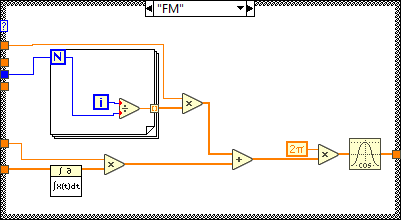
\includegraphics[width=0.9\textwidth]{pic/fm.png}
		\subcaption{Case für die Berechnung eines frequenzmodulierten Signals.}
	\end{subfigure}
	\begin{subfigure}[c]{\textwidth}
		\centering
		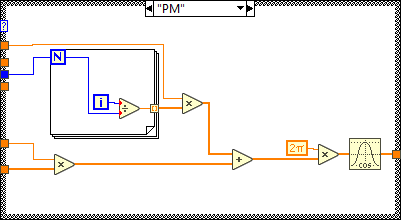
\includegraphics[width=0.9\textwidth]{pic/pm.png}
		\subcaption{Case für die Berechnung eines phasenmodulierten Signals.}
	\end{subfigure}	
	\caption{Alternative Fälle für den Case für die Modulationsart in Abb. \ref{fig:am}.}
	\label{fig:fmpm}	
\end{figure}

\newpage
\pagestyle{empty}
\begin{figure}[H]
	\centering
	\begin{subfigure}[c]{\textwidth}
		\centering
		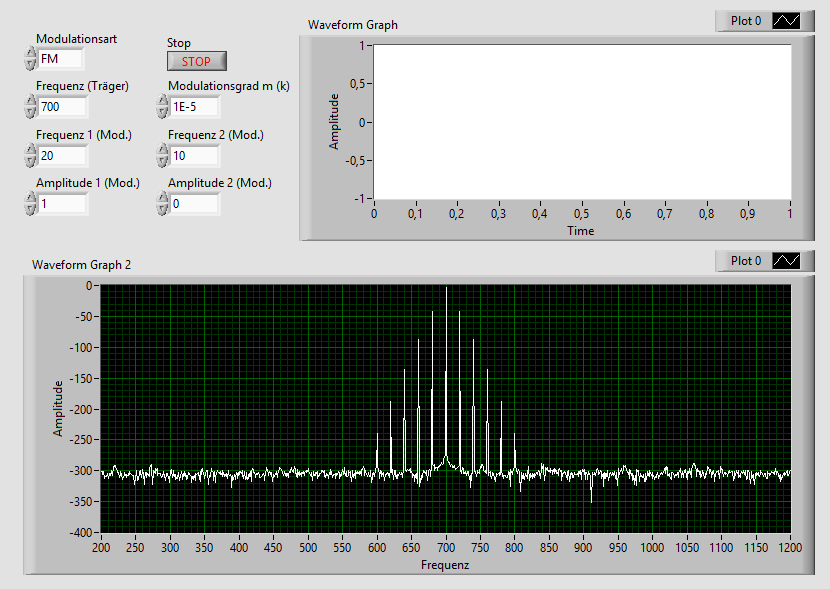
\includegraphics[width=0.9\textwidth]{pic/fm_example.png}
		\caption{Frequenzmodulation}
		\label{fig:fm_example}	
	\end{subfigure}
	\vspace{0.5cm}
	\begin{subfigure}[c]{\textwidth}
		\centering
		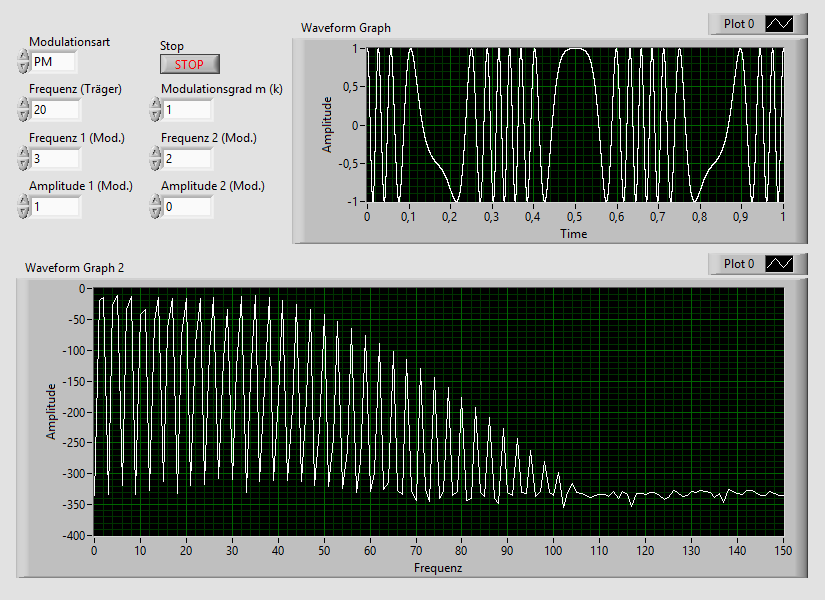
\includegraphics[width=0.9\textwidth]{pic/pm_example.png}
		\caption{Phasenmodulation}
		\label{fig:pm_example}	
	\end{subfigure}
	\caption{Frontpanel des Modulations-VIs bei frequenz- und phasenmoduliertem Signal.}
\end{figure} 

\pagestyle{headings}
Mit dem nun vollständigen Modulations-VI konnten nun auch Signale erzeugt werden, die von der Messstruktur nicht demoduliert werden können.
Die letzte Aufgabe war es die Messstruktur so zu vervollständigen, dass auch frequenz- und phasenmodulierte Signale demoduliert werden können.
Für diese letzte Erweiterung mussten nur zwei weitere Cases eingebaut werden.
Durch ableiten des Signals, wird das zu modulierende Signal ein Teil der Amplitude, weswegen die beiden anderen Modulationstypen mit den gleichen Verfahren demoduliert werden können wie bei der AM.
Abbildung \ref{fig:messstruktur_dafpm} stellt das vollständige Messstruktur-VI dar.
Dieses unterscheidet sich von der Abbildung \ref{fig:messstruktur_dam} nur in den zwei weiteren Cases, der Erweiterung der Speicherfunktion um die Amplituden in den Zeitbildern nach Demodulation/Tiefpass bzw. Bandpass, welcher den Tiefpass ersetzt um ebenfalls den Gleichanteil zu filtern.
	
\

Der erste Case liegt vor der Demodulationsoperation und ist für FM und PM gleich.
Hier wird nur das Signal über ein Express-VI abgeleitet und nach der Konvertierung in diesem VI wieder in eine Waveform zurück konvertiert.
Im Falle der AM geschieht nichts in dem Case, die Kabel gehen also einfach durch diesen durch.
Da nach dem Ableiten bei dem frequenzmodulierten Signal $S_\text{FM}(t)$ das zu modulierende Signal $S(t)$ nun in der Amplitude steht, kann dieses wie ein amplitudenmoduliertes Signal behandelt werden.
	
\

In dem zweiten neuen Case geschieht im Falle der AM und FM also nichts, auch hier verlaufen die Kabel direkt durch den Case.
Bei einem phasenmodulierten Signal befindet sich jedoch nicht das zu modulierende Signal $S(t)$, sondern dessen Ableitung in der Amplitude, weswegen der zweite Case hier genutzt wird, um das Signal einmal zu integrieren, analog zu der Differentiation in dem ersten Case.
Das Frontpanel für ein Beispielsignal ist in Abb. \ref{fig:dpm} dargestellt. 
Wie auch bei den anderen Beispielen sind weitere im Anhang (Abschnitt \ref{sec:anhang}) vorzufinden.

\newpage
\pagestyle{empty}
\begin{figure}[H]
	\centering
	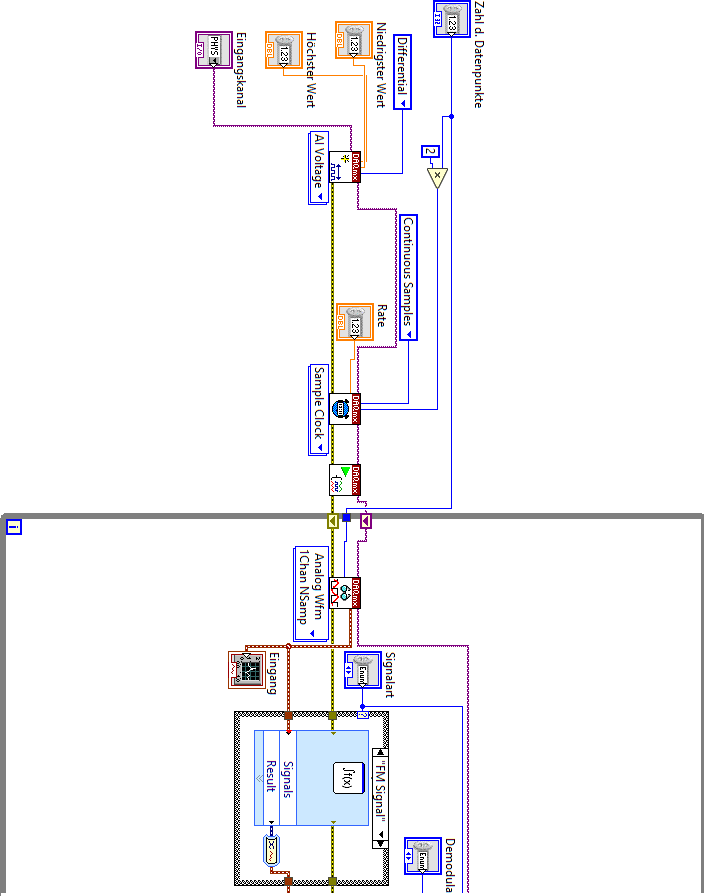
\includegraphics[width=\textwidth]{pic/messstruktur_dafpm1.png}
\end{figure} 
\begin{figure}[H]
	\centering
	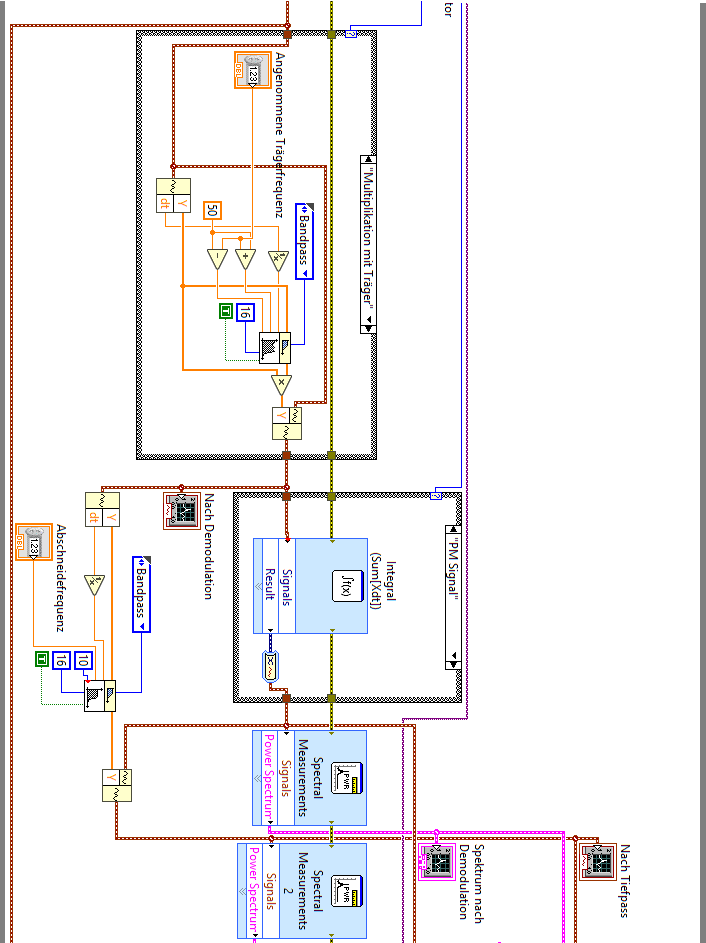
\includegraphics[width=\textwidth]{pic/messstruktur_dafpm2.png}
\end{figure} 
\begin{figure}[H]
	\centering
	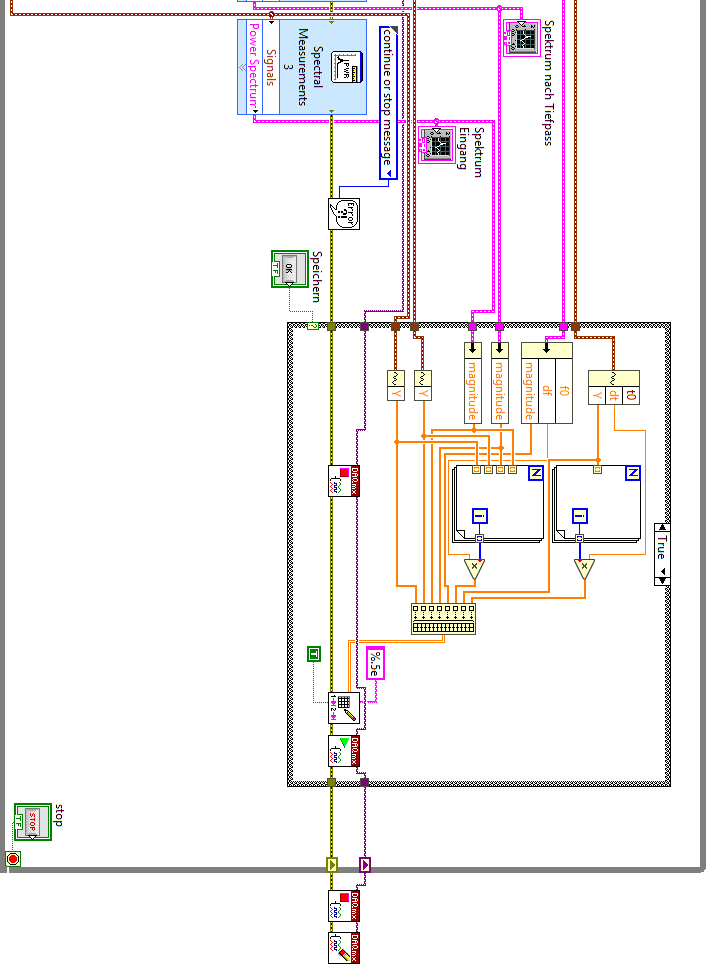
\includegraphics[width=\textwidth]{pic/messstruktur_dafpm3.png}
	\caption{LabVIEW VI der vollständigen Messstruktur mit Demodulationsoptionen für AM, FM und PM, sowie Speicherfunktion.}
	\label{fig:messstruktur_dafpm}	
\end{figure} 

\begin{figure}[H]
	\centering
	\begin{subfigure}[c]{\textwidth}
		\centering
		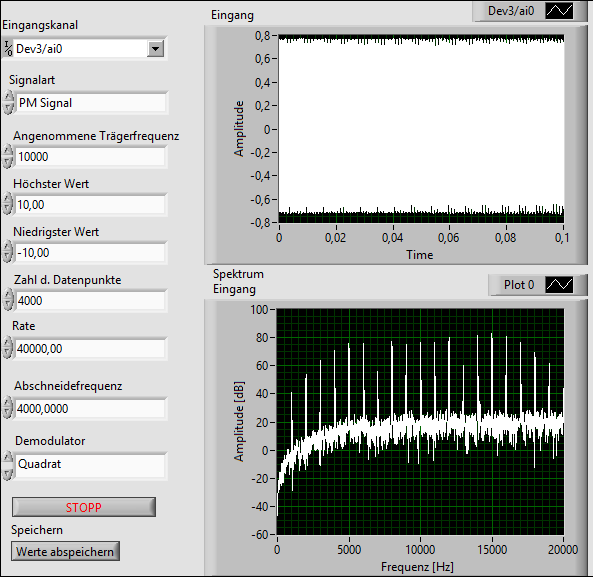
\includegraphics[width=0.7\textwidth]{pic/dpm1.png}
		\subcaption{Linke Seite des Frontpanels mit Parametern und Graphen für das Eingangssignal.}
	\end{subfigure}
	\begin{subfigure}[c]{\textwidth}
		\centering
		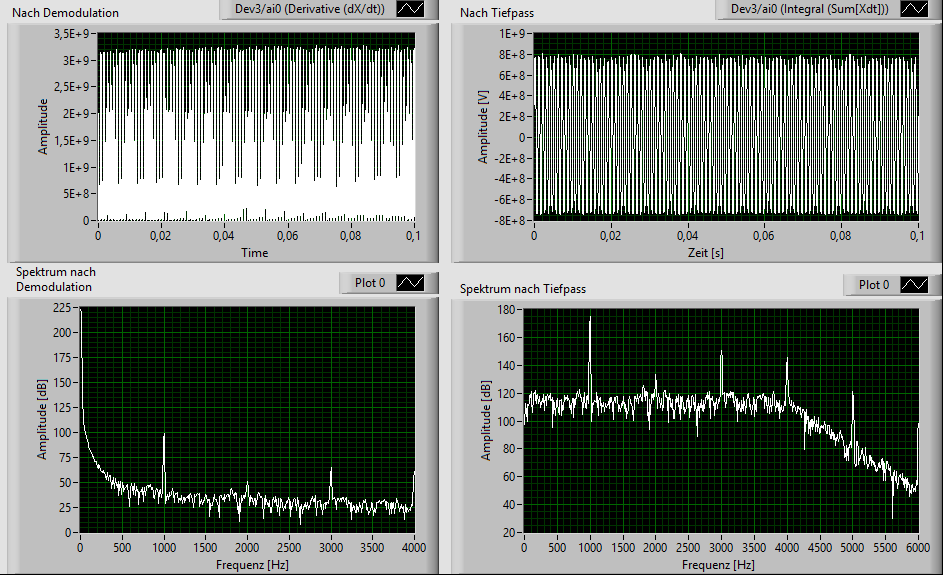
\includegraphics[width=0.9\textwidth]{pic/dpm2.png}
		\subcaption{Rechte Seite des Frontpanels mit Graphen für das demodulierte Signal vor und nach Bandpass.}
	\end{subfigure}	
	\caption{Frontpanel der vollständigen Messstruktur bei eingehendem PM-Signal von dem Modulations-VI.}
	\label{fig:dpm}	
\end{figure} 
\pagestyle{headings}
	}{}

	%\input{tex/name.tex}
	% --- Fazit des gesammten Versuchs einbinden, falls nötig
	\IfFileExists{tex/19_Fazit.tex}{		
		\input{tex/19_Fazit.tex}
	}{}
	
	% --- Anhang einbinden
	\IfFileExists{tex/20_Anhang.tex}{
		\clearpage
		%\appendix
		\section{Anhang}
		\label{sec:anhang}
		\subsection{Bilder zur Amplitudenmodulation}
\pagestyle{headings}
\begin{figure}[H]
	\centering
	\begin{subfigure}[c]{\textwidth}
		\centering
		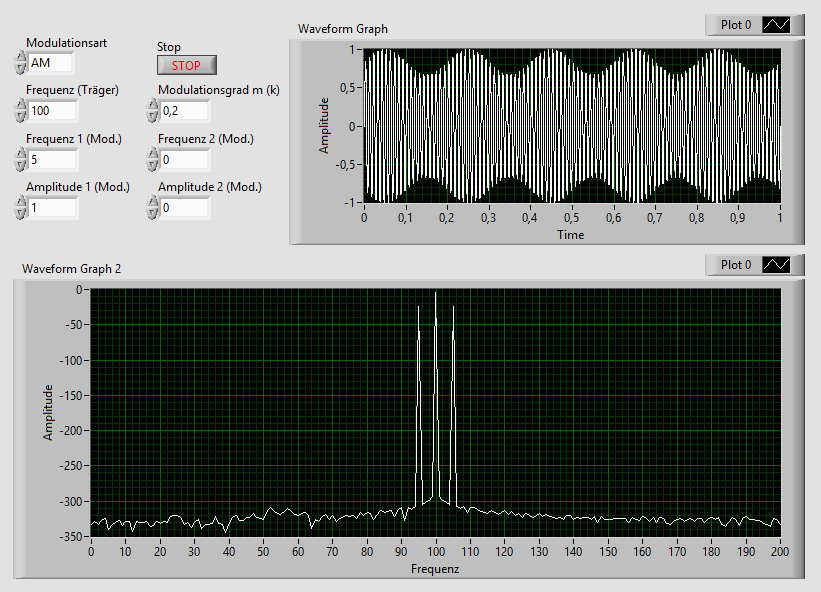
\includegraphics[width=0.7\textwidth]{pic/am_anhang_1.png}
		\subcaption{Modulation mit Trägerfrequenz 100Hz, Mod. Frequenz 5Hz, Mod. Amplitude 1, Modulationsgrad 0,2.}
	\end{subfigure}
	\begin{subfigure}[c]{\textwidth}
		\centering
		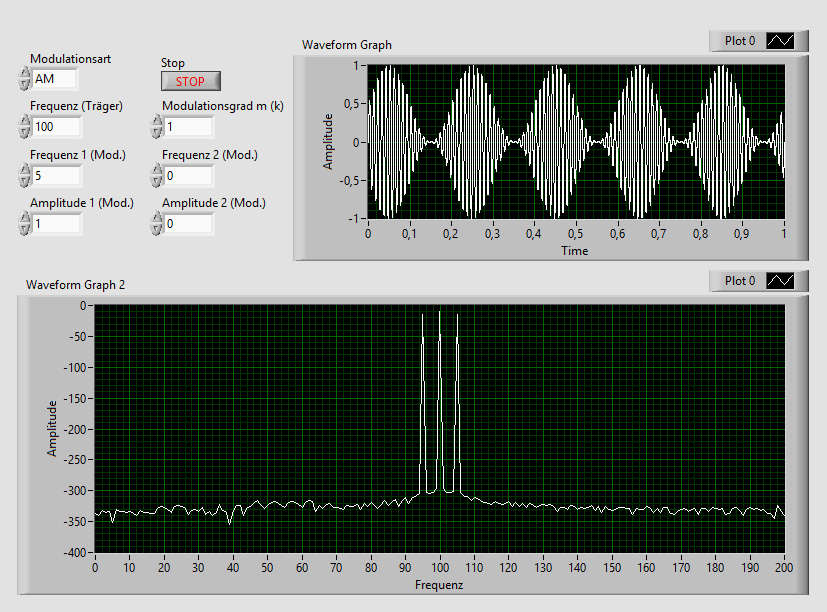
\includegraphics[width=0.7\textwidth]{pic/am_anhang_2.png}
		\subcaption{Modulation mit Trägerfrequenz 100Hz, Mod. Frequenz 5Hz, Mod. Amplitude 1, Modulationsgrad 1.}
	\end{subfigure}	
	\caption{Zwei zusätzliche Beispiele zur Amplitudenmodulation.}
	\label{fig:a1}	
\end{figure}

\subsection{Bilder zur Demodulation von Amplitudenmodulierten Signalen}

\begin{figure}[H]
	\centering
	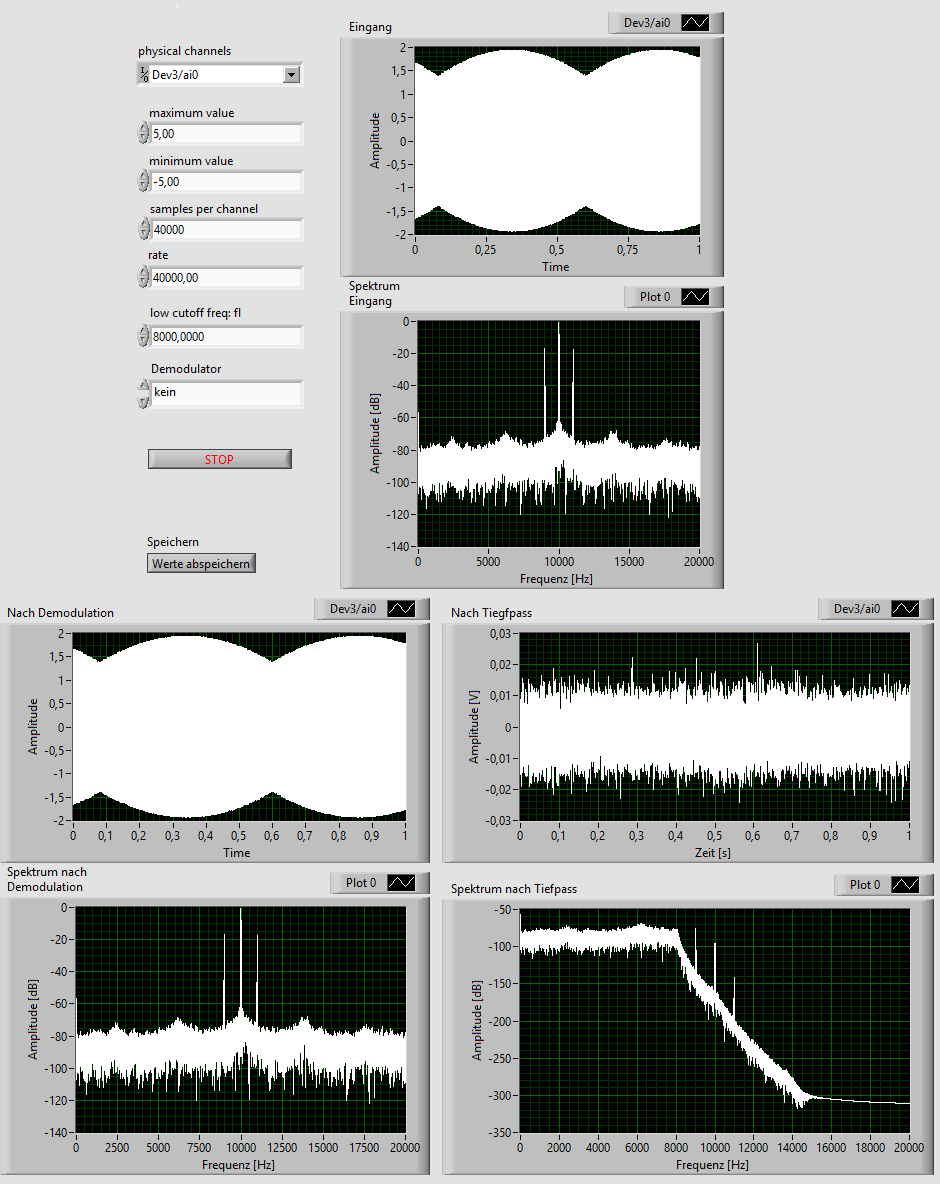
\includegraphics[width=0.9\textwidth]{pic/dam_2_keine.png}
	\caption{Testsignal 2, kein Demodulator.}
	\label{fig:a2}	
\end{figure} 

\newpage

\begin{figure}[H]
	\centering
	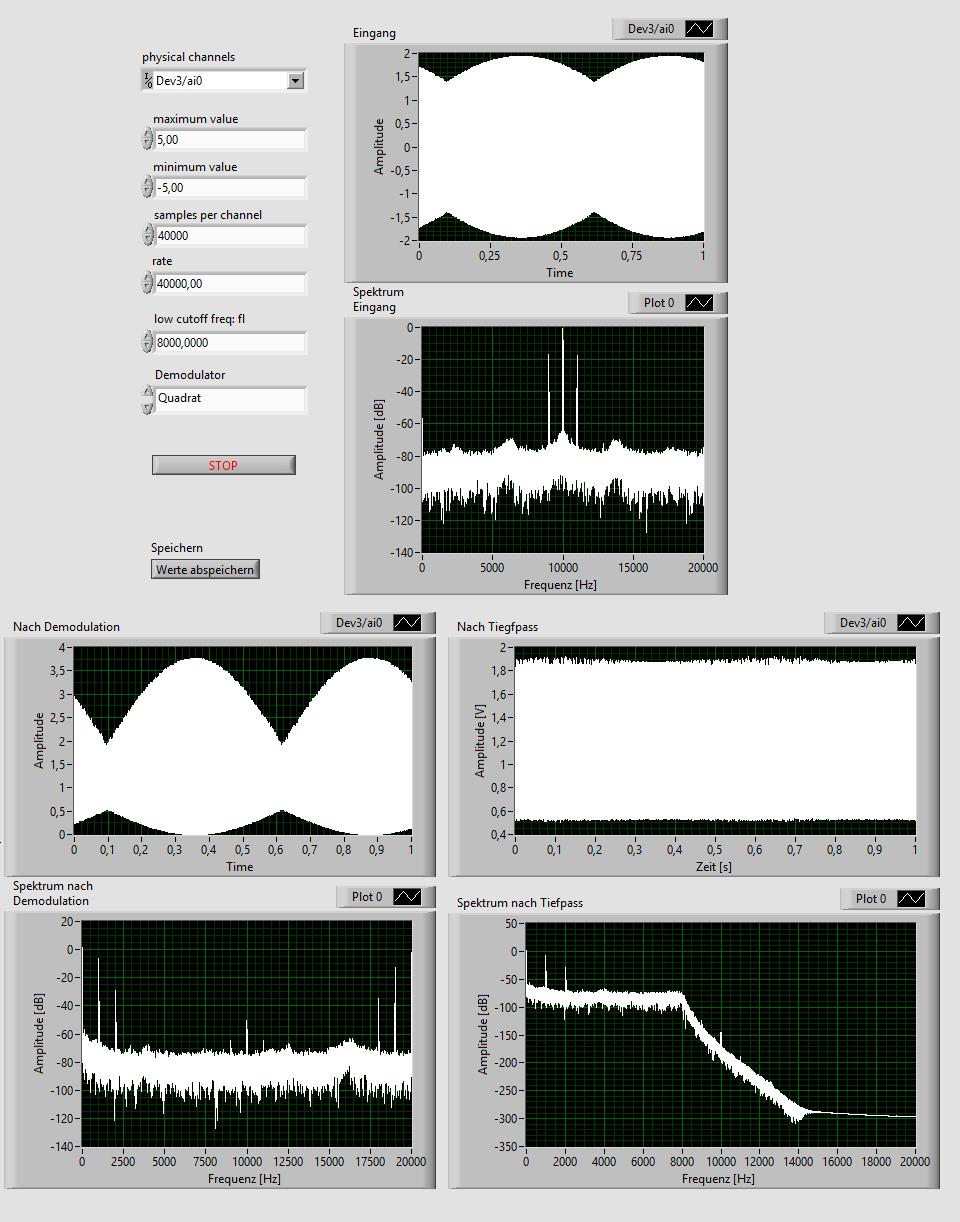
\includegraphics[width=0.9\textwidth]{pic/dam_2_quadrat.png}
	\caption{Testsignal 2, Quadrat. Demodulator.}
	\label{fig:a3}	
\end{figure}

\newpage

\begin{figure}[H]
	\centering
	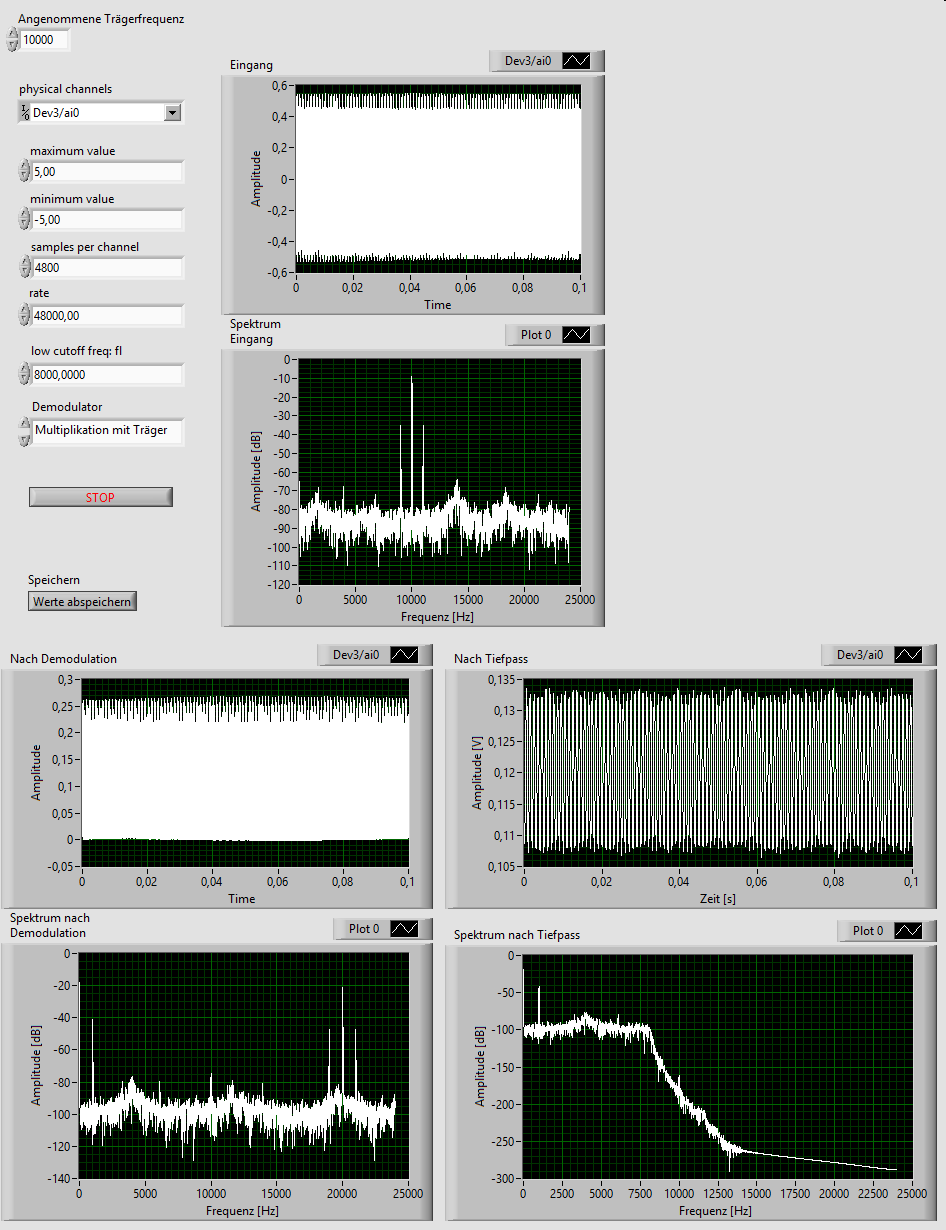
\includegraphics[width=0.9\textwidth]{pic/dam_3_traeger.png}
	\caption{Testsignal 3, Träger. Demodulator.}
	\label{fig:a4}	
\end{figure}

\newpage

\begin{figure}[H]
	\centering
	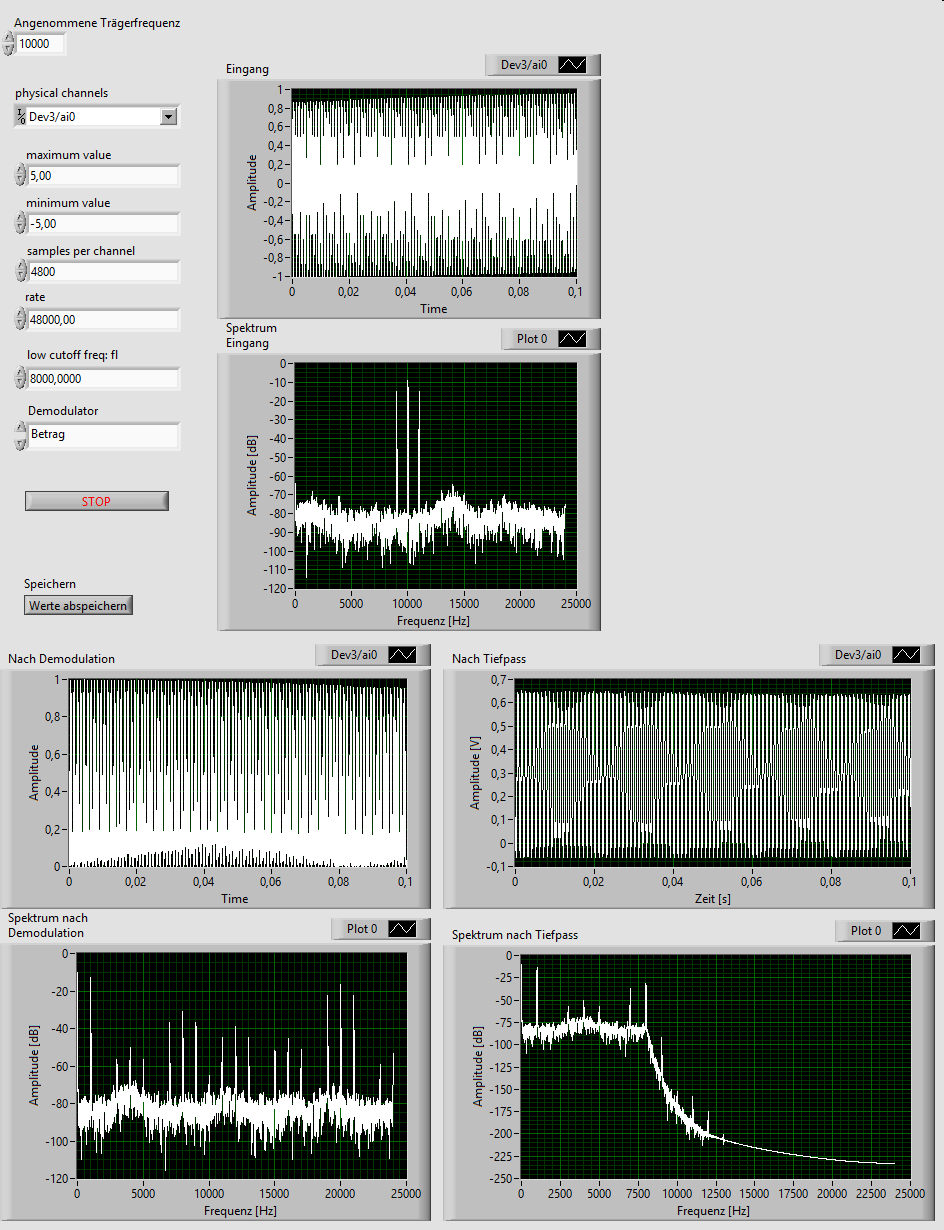
\includegraphics[width=0.9\textwidth]{pic/dam_4_betrag.png}
	\caption{Testsignal 4, Betrag. Demodulator.}
	\label{fig:a5}	
\end{figure}

\newpage

\begin{figure}[H]
	\centering
	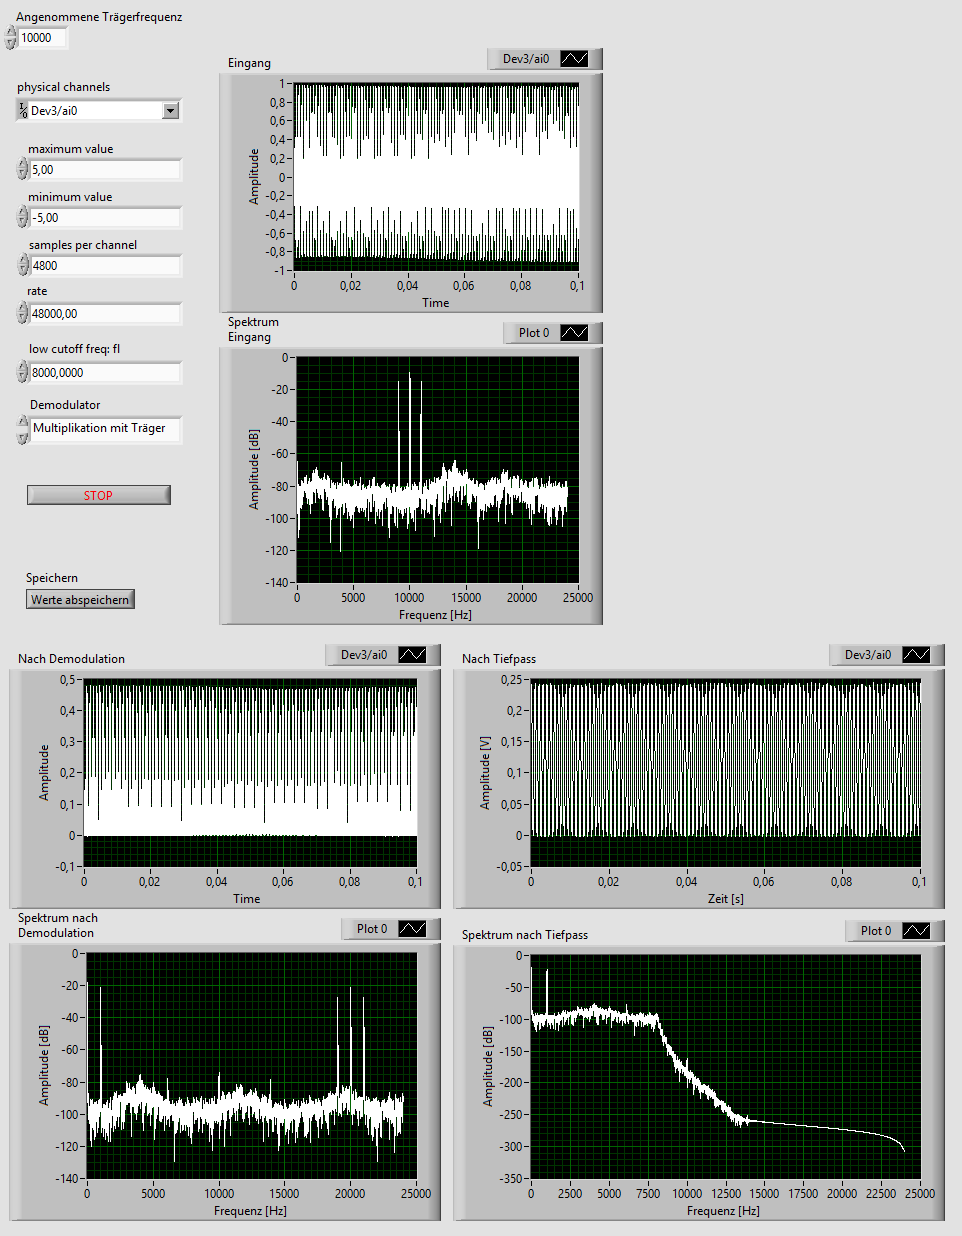
\includegraphics[width=0.9\textwidth]{pic/dam_4_traeger.png}
	\caption{Testsignal 4, Träger. Demodulator.}
	\label{fig:a6}	
\end{figure}

\newpage

\subsection{Bilder zur Frequenzmodulation}

\begin{figure}[H]
	\centering
	\begin{subfigure}[c]{\textwidth}
		\centering
		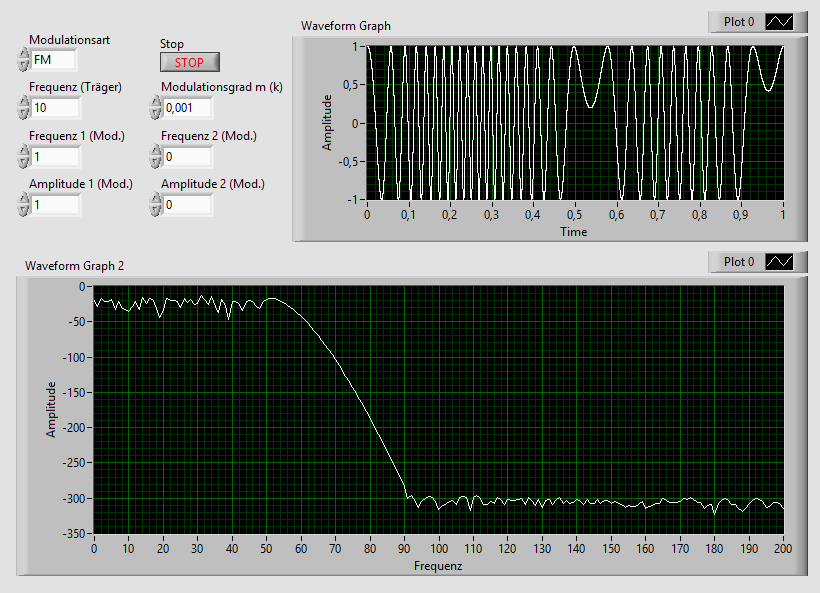
\includegraphics[width=0.7\textwidth]{pic/fmt10.png}
		\subcaption{Trägerfrequenz 10 Hz, Mod. Frequenz 1 Hz, Mod. Amplitude 1, Modulationsgrad 0,001.}
	\end{subfigure}
	\begin{subfigure}[c]{\textwidth}
		\centering
		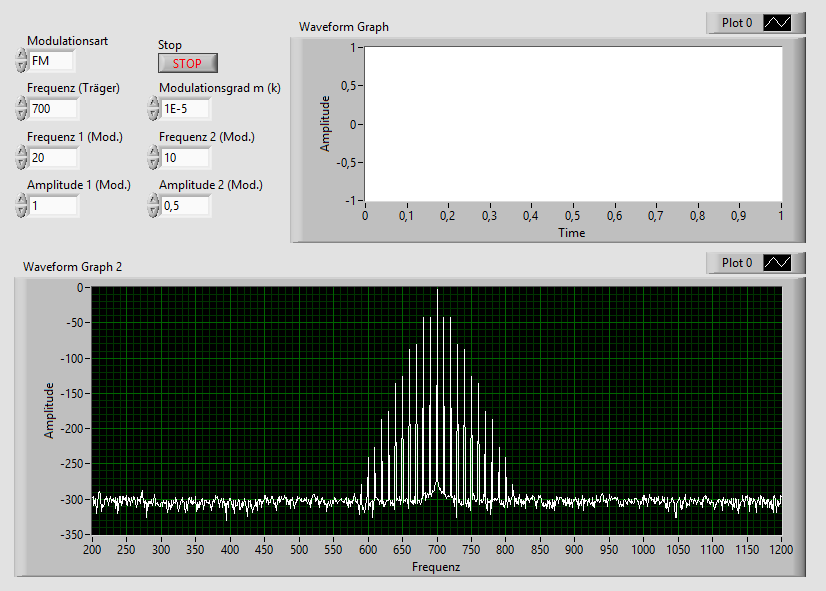
\includegraphics[width=0.7\textwidth]{pic/fmt700.png}
		\subcaption{Trägerfrequenz 700 Hz, Mod. Frequenz 10 Hz und 20 Hz, Mod. Amplitude 0,5 und 1, Modulationsgrad $10^{-5}$.}
	\end{subfigure}	
	\caption{Zwei zusätzliche Beispiele zur Frequenzmodulation.}
	\label{fig:a7}	
\end{figure}


\newpage

\subsection{Bilder zur Phasenmodulation}

\begin{figure}[H]
	\centering
	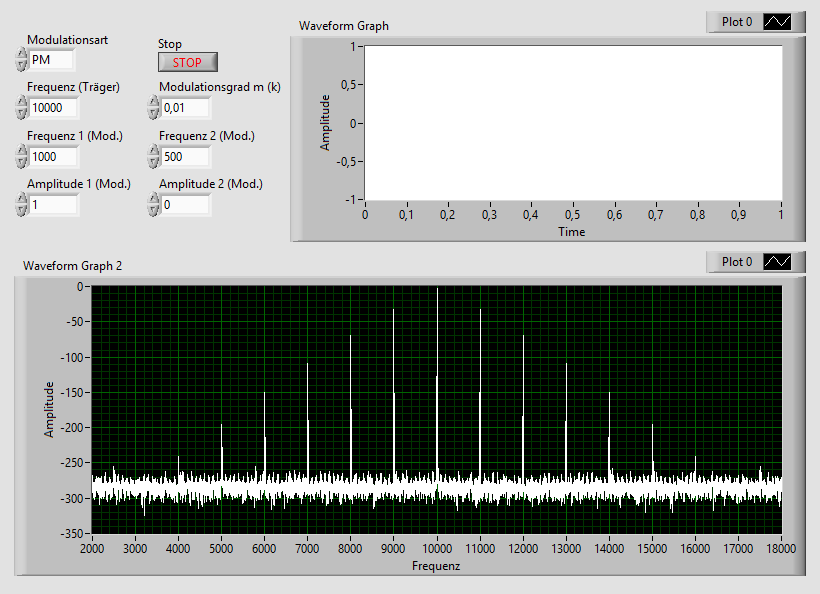
\includegraphics[width=0.7\textwidth]{pic/t10km1kg001.png}
	\caption{Weiteres Beispiel zur Phasenmodulation. Die Parameter können der Abbildung entnommen werden.}
	\label{fig:a8}	
\end{figure} 

\begin{figure}[H]
	\centering
	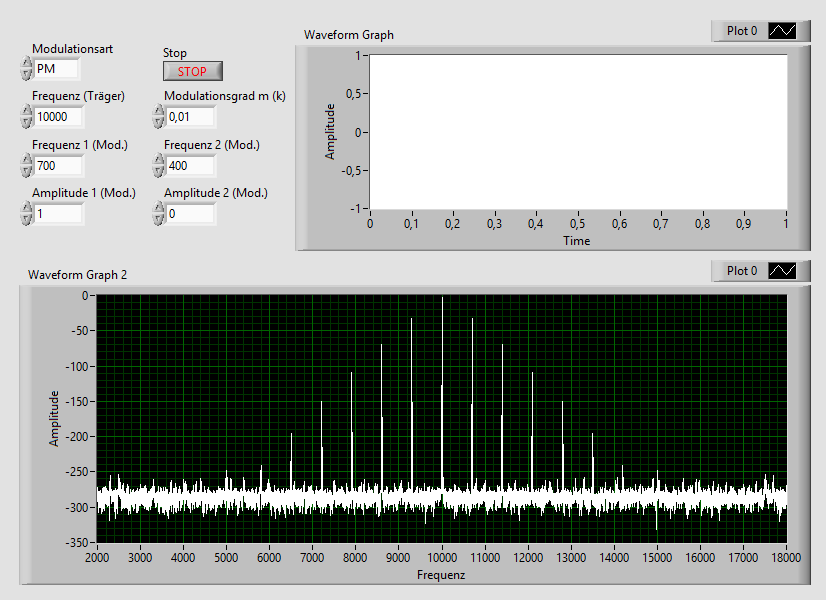
\includegraphics[width=0.7\textwidth]{pic/t10km700g001.png}
	\caption{Weiteres Beispiel zur Phasenmodulation. Die Parameter können der Abbildung entnommen werden.}
	\label{fig:a9}	
\end{figure} 

\begin{figure}[H]
	\centering
	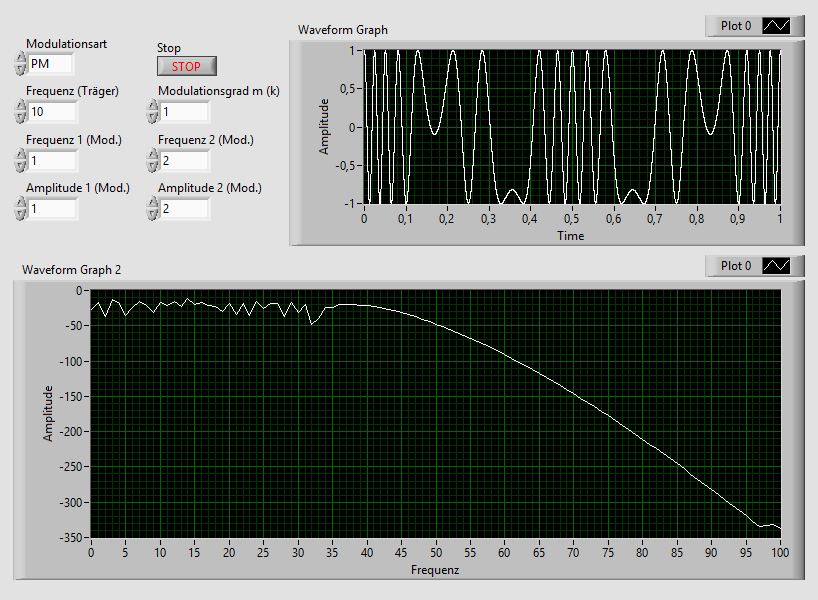
\includegraphics[width=0.7\textwidth]{pic/t10m1-2g1.png}
	\caption{Weiteres Beispiel zur Phasenmodulation. Die Parameter können der Abbildung entnommen werden.}
	\label{fig:a10}	
\end{figure} 
\begin{figure}[H]
	\centering
	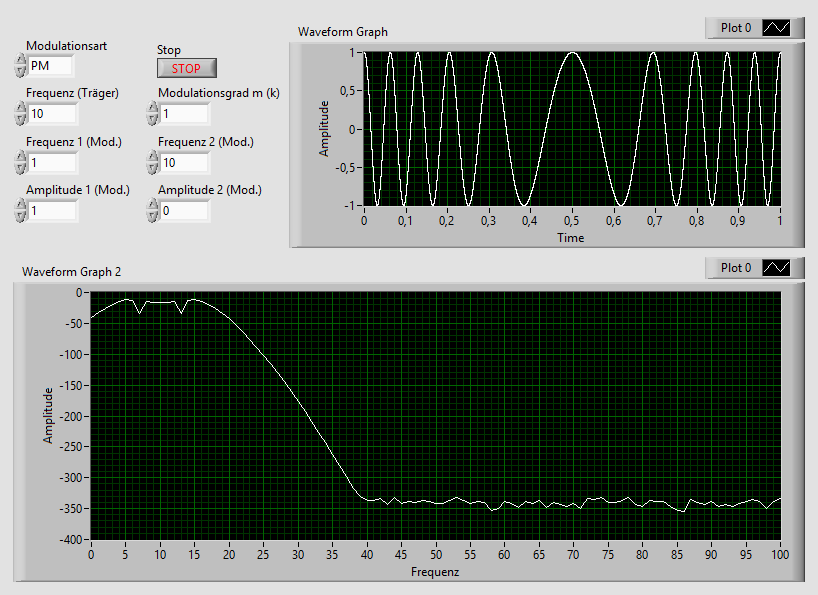
\includegraphics[width=0.7\textwidth]{pic/t10m1g1.png}
	\caption{Weiteres Beispiel zur Phasenmodulation. Die Parameter können der Abbildung entnommen werden.}
	\label{fig:a11}	
\end{figure} 

\newpage

\begin{figure}[H]
	\centering
	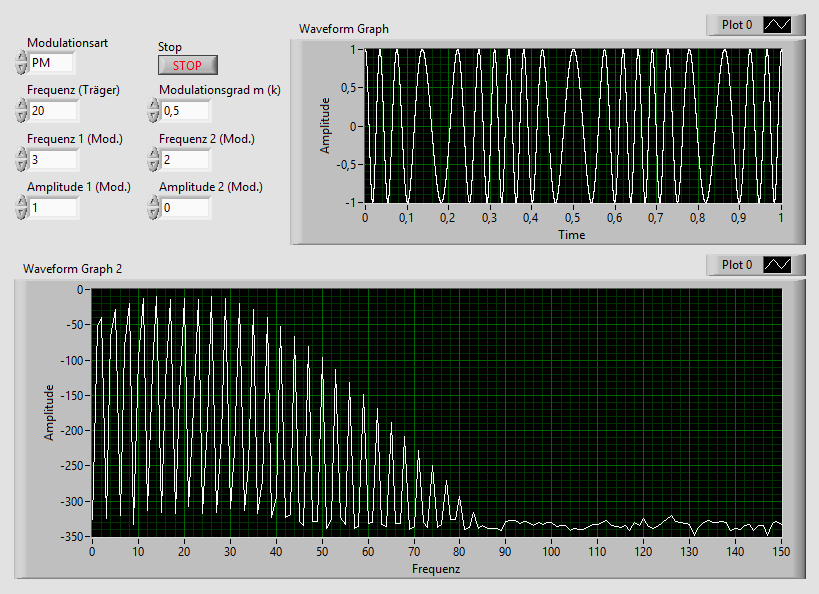
\includegraphics[width=1\textwidth]{pic/t20m3g05.png}
	\caption{Weiteres Beispiel zur Phasenmodulation. Die Parameter können der Abbildung entnommen werden.}
	\label{fig:a12}	
\end{figure} 
\subsection{Bilder zur Demodulation von Frequenz- und Phasenmodulierten Signalen}

\begin{figure}[H]
	\centering
	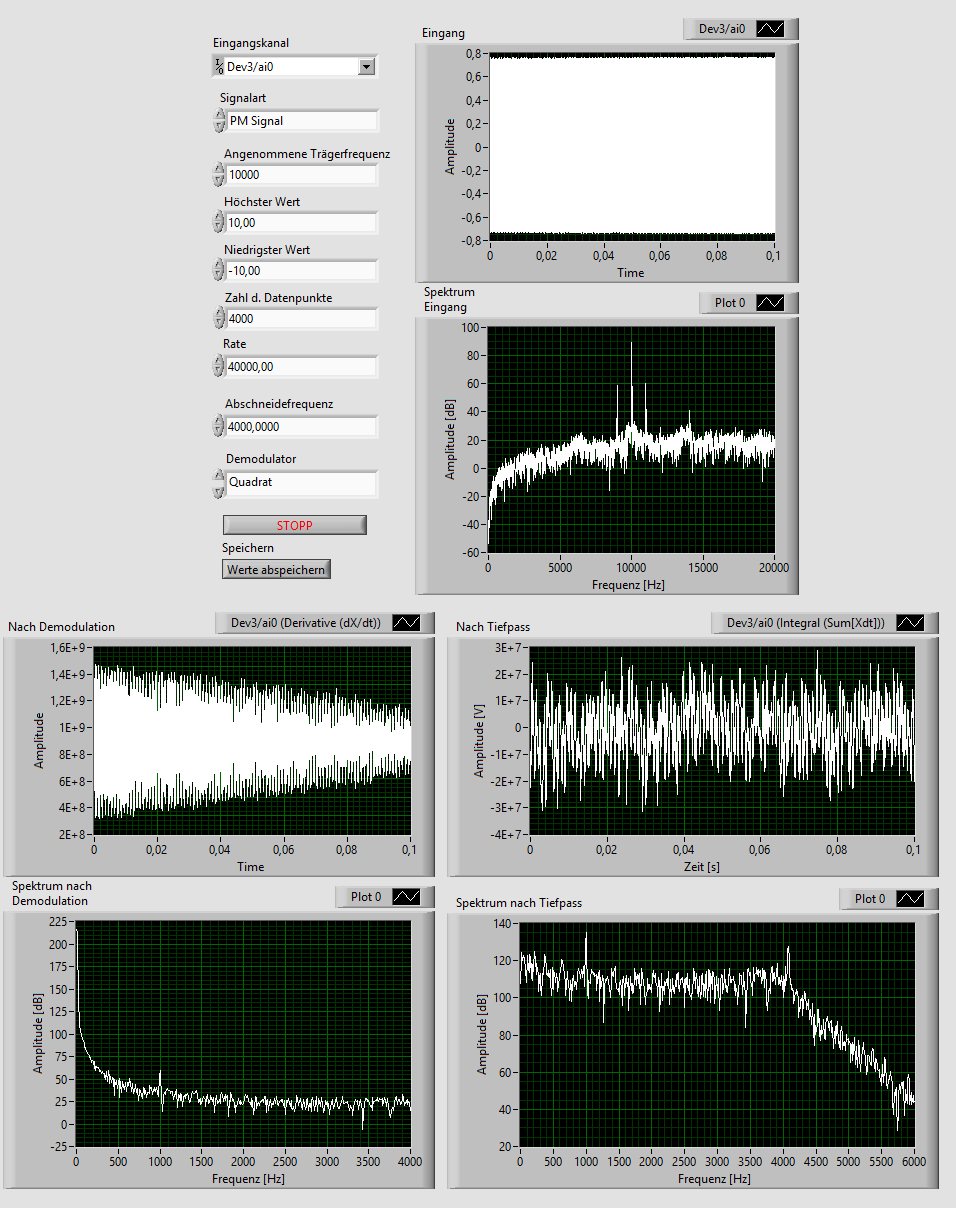
\includegraphics[width=0.8\textwidth]{pic/PM10k1k001.png}
	\caption{Weiteres Beispiel zur Demodulation eines Phasenmodulierten Signals. Die Parameter können der Abbildung entnommen werden.}
	\label{fig:a13}	
\end{figure} 

\begin{figure}[H]
	\centering
	\includegraphics[width=1\textwidth]{pic/FM10k1k1.png}
	\caption{Weiteres Beispiel zur Demodulation eines Frequenzmodulierten Signals. Die Parameter können der Abbildung entnommen werden.}
	\label{fig:a14}	
\end{figure} 

\begin{figure}[H]
	\centering
	\includegraphics[width=1\textwidth]{pic/FM10k1k001.png}
	\caption{Weiteres Beispiel zur Frequenzmodulation. Die Parameter können der Abbildung entnommen werden.}
	\label{fig:a15}	
\end{figure} 


	}{}
	
	% --- Literaturverzeichnis mit BibLaTeX
	 \ifthenelse{\boolean{showBibliography}}{
		\clearpage
		\printbibliography
	}{}
	
\end{document} 
